% Chapter 1

\chapter{Introduction} % Main chapter title

\label{Chapter1} % For referencing the chapter elsewhere, use \ref{Chapter1} 


%----------------------------------------------------------------------------------------

% Define some commands to keep the formatting separated from the content 

%----------------------------------------------------------------------------------------

Artificial Neural Networks and other optimization-based general
function approximation models are the core of modern
machine learning \cite{prakash2018}. These models have dominated competitions in image processing, optical character recognition, object detection, video classification, natural language processing, and many other fields \cite{SCHMIDHUBER201585}. All such modern models are
trained via gradient-based optimization, e.g. Stochastic Gradient Descent (SGD) with
gradients computed via back propagation. \cite{goodfellow2013multidigit}. Although the performance of these models is practically
miraculous within the training and testing context for which they are designed, they have a few intriguing properties. It was discovered in 2013 
\cite{Szegedy2013} that images can be generated
which apparently trick such models in a classification context in  difficult-to-control ways \cite{Khoury2018}. The intent of this
research is to investigate these \emph{adversarial examples} in a
mathematical context and use them to study pertinent 
properties of the learning models from which they arise.

\subsection{Artificial Neural Networks (ANNs)}

%\subsection{A Brief History of Neural Networks (NNs)}

The history of Neural Networks begins in the field of Theoretical Neuropsychology with a much-cited paper by McCulloch and Pitts in which they describe the mechanics of cognition in the context of computation \cite{mcculloch1943logical}. This initial framework for computational cognition did not include a notion for learning, but the following decade brought the concept of learning (as optimization) and many simple NNs (linear regression models applied to computational cognition). The perceptron, the most granular element of a neural network, was proposed in another much-cited paper by Rosenblatt in 1958 \cite{rosenblatt1958perceptron}, and multilevel (deep) networks were proposed by 1965 in a paper by Ivakhnenko and Lapa \cite{ivakhnenko1965cybernetic}. 

By the 1960s, these neural network models became disassociated from the cutting-edge of cognitive science, and interest had shifted to their application in modeling and industrial computation. The hardware limitations of the time served as a significant barrier to wider application and the concept of the "neural network" was sometimes treated as a solution looking for a problem. Compounding these limitations was a significant roadblock published by Minsky and Papert in 1969: A proof that basic perceptrons could not encode exclusive-or \cite{minsky1969perceptrons}. As a result, interest in developing neural network theory waned. The next necessary step in the development of modern neural network models was an advance that would allow them to be trained efficiently with computing power available. Learning methods required a gradient, and the technique necessary for computing gradients of large-scale multi-parameter models was apparently proposed in a 1970 in a Finnish masters thesis \cite{linnainmaa1970representation}. Techniques from control theory were applied to develop a means of propagating error backward through models which could be described as directed graphs. The idea was applied to neural networks by a Harvard student Paul Werbos\cite{werbos1974beyond} and refined in later publications. 

The final essential puzzle piece for neural network models was to take advantage of their layered structure, which would allow backpropagation computations at a given layer to be done in parallel. This key insight, indeed the core of much of modern computing, was a description of parallel and distributed processing in the context of cognition by Rumelhard and McClelland in 1986 \cite{mcclelland1986parallel} with an astonishing 22,453 citations (a number that grows nearly every day). With these pieces in place, the world was ready for someone to finally apply neural network models to a relevant problem. In 1989, Yann LeCun and a group at Bell Labs managed to do just that. LeCun  refined backpropagation into the form it is used today \cite{lecun1989backpropagation}, invented Convolutional Neural Networks \ref{cnn} \cite{lecun1995convolutional}, and by 1998, he had worked with his team to implement what has  become the industry standard for banks to recognize hand-written numbers on checks \cite{lecun1998gradient}. 

Starting in the 2000s, neural networks have blown up in scale and application, so it's harder to keep track of the discrete historical developments. Most of the progress in terms of performance and application has come from contests (e.g: \url{http:/image-net.org/challenges/LSVRC/}) in which a bounty (or publicity) is offered and labs around the world compete to build a network which solves the competition's problem. Schimdhuber's group \cite{SCHMIDHUBER201585}, and a similar group at Google have dominated many of these competitions. The cutting-edge today is represented by networks like Inception v4 designed by Google for image classification  which contains approximately 43 million parameters  \cite{Szegedy2013}. Early versions of this network took 1-2 million dollars worth of compute-time to train. ANNs now appear in nearly every industry from devices which use ANNs to intelligently adapt their performance, to the sciences which rely on ANNs to eliminate tedious sorting and identification of data that previously had to be relegated to humans.

\subsection{Structure}
In this subsection we give a mathematical description of artificial neural networks. 

%TODO: change this definition to something very vague and general -- use wikipedia 
A \emph{neuron} is a nonlinear operator that takes input in $\R^n$ to $\R$, historically designed to emulate the activation characteristics of an organic neuron. A collection of neurons that are connected via a (usually directed) graph structure are known as an \emph{Artificial Neural Network (ANN)}. 
%\begin{definition}{Artificial Neural Networks (ANNs)} are functions $N:\R^n \to \R^m$ determined by weighted directed graphs whose nodes compose a weighted sum of the input along each incoming edge with the weights for those edges with a nonlinear activation function to generate an output. We can denote an ANN as a function in terms of an input vector $\vec x$ and its parameters $\vec w$: $N(\vec x, \vec w)$.  
%\end{definition}

The fundamental building blocks of most ANNs are artificial neurons which we will refer to as \emph{perceptrons}.

\begin{definition}{A \textbf{Perceptron} is  }
\label{perceptron}
a function $P_{\vec w}: \R^n \to \R$ which has \emph{weights} $\vec
w \in \R^n$ corresponding with each element of an input vector $\vec
x\in \R^n$ and a bias $b \in \R$:
\[P_{\vec w}(\vec x) = f(\left(\ip{\vec w,\vec x} + b\right)\]
\[P_{\vec w}(\vec x) = f\left(b + \sum_{i = 1}^n w_i x_i\right)\]
where $f: \R \to \R$ is continuous. The function $f$ is called the \textbf{activation function} for $P$. 
\end{definition}


The only nonlinearity in $P_w$ is contained in $f$. If $f$ is chosen to be linear, then $P$ will be a linear operator. Although this has the advantage of simplicity, linear operators do not perform well on nonlinear problems like classification. For this reason, activation functions are generally chosen to be nonlinear. Historically, heaviside functions were used for activation, later replaced with sigmoids \cite{malik1990preattentive} for their smoothness, switching structure, and convenient
compactification of the output from each perceptron.  It was recently discovered that a simpler nonlinear function, the \emph{Rectified Linear Unit (ReLU)} works as well or better in most neural-network-type applications \cite{glorot2011deep} and additionally training algorithms on ReLU activated networks converge faster \cite{nair_rectified_nodate}. 

\begin{definition}{The Rectified Linear Unit (ReLU) function is}
\label{relu}

  \[\relu(x) = \begin{cases} 0, & x \leq 0;\\
      x, & x > 0,\end{cases}\]
\end{definition}


The single nonlinearity of this activation function
at $x = 0$ is sufficient to guarantee existence of $\epsilon$ approximation of smooth functions by an ANN composed of sufficiently numerous perceptrons connected by ReLU \cite{petersen2018optimal}. In addition, ReLU is convex, which enables efficient numerical approximation of smooth functions in shallow networks  \cite{li2017convergence}.  


% \cite{prakash2018}
% \cite{Szegedy2013}
% \cite{goodfellow_explaining_2014}
% \cite{Bishop:2006:PRM:1162264}
% \cite{mohammad16}
% \cite{Khoury2018}
% \cite{inevitable2018}
% \cite{tsipras2018robustness}

% step 1 intro (2 slides) motivating picture and overview
% step 2 liu key point is that you really don't need to know much
% about the distribution for the depth sampling to approximate it well
% (2 slides define depth and show key theorem)
% step 3 natural algorithm (1 slide)
% step 4 (2 slides) better algorithm (2 slides + board work)
% step 5 (1 slide) computation time for different algorithms
% step 6 (1 slide) extension to n-dimensional simplices
% step 7 (1 slide) wrap up with final clean examples with bands. We
% want to do with clustering what they did with uncertainty. 

%%%%%%%%%%%%%%%%%%%%%%%%%%%%%%%%%%%%%%%%%(1)


%  \subsubsection{Definitions}
% The model is named for its proxy in the human brain and we call the 
% units of this model \emph{neurons} which function much like biological
% neurons. We define a neuron (node) in a neural network as an operation
% on an input vector $x \in \R^n$ with a set of weights $w(i,j,k)$ for
% each element of the input, a bias $b(i,j)$, and an activation filter
% $g_i: \R \to \R$ which will generate an output signal from the neuron
% (in general practice, the activation filter is consistent across the
% entire network or over groups of neurons, but it can vary for each
% neuron if desired). The activation filter will contain any
% non-linearity for the model.  
% \begin{tcolorbox}{Neuron (Node)}
% \[N_{i,j}(x) = g_i\left(b_{i,j} + \sum_{k = 1}^n w_{i,j,k} x_k\right)\]
% \end{tcolorbox}

% Output filters are generally designed to squeeze the raw output from a
% neuron into a convenient decision space: boolean or  sigmoidal output. \\
% \begin{tcolorbox}{Output Filter Examples}
% \[g_i(N_{i,j}(x)) = \begin{cases} 1 , & \text{ if } N_{i,j}(x) > \e\\
% 0 , & \text{ if } N_{i,j}(x) \leq \e\end{cases}\]
% or
% \[g_i(N_{i,j}(x)) = \frac{1}{1 + e^{N_{i,j}(x) - M_{i,j}}}\]
% (where $M_{i,j}$ is an expectation for $N_{i,j}$)
% \end{tcolorbox}


In general ANNs 
must not be cyclic and, for convenience, are often arranged into
independent layers. An early roadblock for neural networks was a proof by Minsky \cite{minsky1969perceptrons} that single layers of perceptrons could not encode exclusive-or. Depth, the number of layers in a neural network, is a key factor in its ability to approximate complicated functions including exclusive-or \cite{kak1993training}. For this reason, modern ANNs are usually composed of many layers (3-100). The most common instance of a neural network model is a fully connected \emph{feed forward (FF)} configuration. In this configuration data enters as an input layer which is fed into each of the nodes in the first layer of neurons. Output of the first layer is fed into each of the nodes in the second layer, and so on until the output of the final layer is fed into an output filter which generates the final result of the neural network. 




In this example of a FF network, an input vector in $\R^7$ is mapped to a
an output in $\R^3$ which is fed into a classifier. Each blue circle
represents a perceptron with the ReLU activation function. 

% \begin{figure}[H]
%   \centering
%   \caption{BoxPlot Uncertainty}
%     \includegraphics[width=12cm]{BoxPlot_Uncertainty.png}
% \end{figure}
% \centering \footnotesize{Images produced by Mirzargar et al \cite{Raj2017}}

\scalebox{.9}{
\begin{tikzpicture}[shorten >=1pt,->,draw=black!50, node distance=\layersep]
    \tikzstyle{every pin edge}=[<-,shorten <=1pt]
    \tikzstyle{neuron}=[circle,fill=black!25,minimum size=9pt,inner sep=0pt]
    \tikzstyle{input neuron}=[neuron, fill=green!50];
    \tikzstyle{output neuron}=[neuron, fill=red!50];
    \tikzstyle{hidden neuron}=[neuron, fill=blue!50];
    \tikzstyle{annot} = [text width=4em, text centered]

    % Draw the input layer nodes
    \foreach \name / \y in {1,...,7}
    % This is the same as writing \foreach \name / \y in {1/1,2/2,3/3,4/4}
        \node[input neuron] (I-\name) at (0,-\y) {};
%pin=left:Input \#\y
    % Draw the hidden layer nodes
    \foreach \name / \y in {1,...,6}
        \path[yshift=-0.5cm]
            node[hidden neuron] (H-\name) at (\layersep,-\y cm) {};

    \foreach \name / \y in {1,...,4}
        \path[yshift=-1.5cm,xshift=2.0cm]
            node[hidden neuron] (HH-\name) at (\layersep,-\y cm) {};

    \foreach \name / \y in {1,...,3}
        \path[yshift=-2cm,xshift=4.0cm]
            node[output neuron] (O-\name) at (\layersep,-\y cm) {};

    % Draw the output layer node
%   \foreach \name / \y in {1,...,3}
%        \path[yshift=-1.5cm,xshift=4.0cm]
%            \node[output neuron] (O-\name) at (\layersep,-\y cm) {};


    % Connect every node in the input layer with every node in the
    % hidden layer.
    \foreach \source in {1,...,7}
        \foreach \dest in {1,...,6}
            \path (I-\source) edge (H-\dest);

    \foreach \source in {1,...,6}
        \foreach \dest in {1,...,4}
            \path (H-\source) edge (HH-\dest);

    % Connect every node in the hidden layer with the output layer
    \foreach \source in {1,...,4}
        \foreach \dest in {1,...,3}
            \path (HH-\source) edge (O-\dest);

    % Annotate the layers
  \node [rectangle, draw, minimum height=6.2cm, text width=.8cm, text
  centered, left =.8cm of I-4] (mm) {Data};

    \foreach \source in {1,...,7}
        \path [line] (mm.east|-I-\source) -- (I-\source);

    \node[annot,above of=H-1, node distance=2cm] (hl) {Layer 1};
    \node[annot,left of=hl] {Input };
    \node[annot,right of=hl] (h3) {Layer 2} ;
    \node[annot,right of=h3] {Output Layer};
  \node [rectangle, draw, minimum height=5cm, text width=1.6cm, text
  centered, right =6.8cm of I-4] (mc) {Classifier};
    \foreach \source in {1,...,3}
        \path [line] (O-\source) -- (mc.west|-O-\source);


\end{tikzpicture}
}

%%%%%%%%%%%%%%%%%%%%%%%%%%%%%%%%%%%%%%%%%%%%%%%%%%%%%%%%%%%%%%%%

%%%%%%%%%%%%%%%%%%%%%%%%%%%%%%%%%%%%%%%%%%%(2)
% 2. define classifier

The output of this ANN is fed into a classifier. To complete this
example, we can define the most common classifier, Softmax:


\begin{definition}{Softmax (or the normalized exponential) is the function given by}
\[s : \R^n \to [0,1]^n\]
\[s_j(\vec x) = \frac{e^{x_j}}{\sum_{k = 1}^n e^{x_k}}\]
\end{definition}

\begin{definition}{We can define a classifier which picks the class corresponding with the largest output element from Softmax: }
\[\text{(Output Classification)  }   c_s(\vec x) = \text{argmax}_{i} s_i(\vec{x})\]
\end{definition}
% It is important that the classifier admit a directed error function
During training, the output $y \in \R^n$ from a network can thus be compressed using softmax into $[0,1]^n$ as a surrogate for probability for each possible class or directly into the classes which we can represent as the simplex for the vertices of $[0,1]^n$. 

\cite{Bishop:2006:PRM:1162264}

\subsubsection{Convolutional Neural Networks (CNNs)}\label{cnn}

Another common type of neural network which is a component in many modern applications including one in the experiments to follow are Convolutional Neural Networks (CNNs). CNNs are fundamentally composed of
perceptrons, but each layer is not fully connected to the
next. Instead, layers are arranged spatially and overlapping groups of perceptrons are independently connected to the nodes of the next layer, usually with a nonlinear filter that computes the maximum of all of the incoming nodes to a new node. This structure has been shown to be very effective on problems with spatial information \cite{lecun1995convolutional}. 

\subsection{Training ANNs}

Neural networks consist of a very large number of perceptrons with many parameters. Directly solving the system implied by these parameters and the empirical risk minimization problem defined below would be difficult, so we must use a
modular approach which takes advantage of the simple and regular structure of ANNs.

 A breakthrough came with the application of techniques derived from control theory to ANNs in the late 1980s \cite{rumelhart1986learning}, dubbed backpropagation. This technique was refined into its modern form in the thesis and continuing work of Yann LeCun \cite{lecun1988theoretical}. In this method, error is propagated backward taking advantage of the directed structure of the network to compute a gradient for each parameter defining it. Because modern ANNs are usually separated into discrete layers, gradients can be computed in parallel for all perceptrons at the same depth of the network
\cite{Bishop:2006:PRM:1162264}. Leveraging modern GPUs and parallel computing technologies, these gradients can be computed very quickly. There are a number of important considerations in training. We discuss a few in the following subsections. 

\subsubsection{Selection of the Training Set}

The first step in training an ANN is the selection of a training set. ANNs fundamentally are universal function approximators: Given a set of input data and corresponding output data, they approximate a mapping from one to the other. Performance is dependent on how well the phenomenon we hope to model is represented by the training data. The training data must consist of a set of inputs (e.g., images) and a set of outputs (e.g., labels) which contain sufficient examples to characterize the intended model. In a way, this is how we pose a question to the neural network. One must always ask whether the question we wish to pose is well-expressed by the training data we have available. 

The most important attributes of a training dataset are the number of
samples it contains and its density near where the model will be making predictions. According to conventional wisdom, training a neural network with $K$ parameters
will be very challenging if there are fewer than $K$ training samples
available. The modular structure of ANNs can be combined with regularization of the weights to overcome these limitations \cite{liu2015very}. 
In general, we will denote a training set by $(X,Y)$ where $X$ is an indexed set of inputs and $Y$ is a corresponding indexed set of labels. 

\subsubsection{Selecting a Loss Function}

Once we have selected a set of training data (both inputs and outputs), we must decide how we will evaluate the match between the ANNs output and the defined outputs from the training dataset -- we will quantify the deviation of the ANN compared with the given correspondence as a Loss. In general \emph{loss functions} are nonzero functions which compare an output $y$ against a ground-truth $\hat y$. Generally they have the property that an ideal outcome would have a loss of 0. 

One commonly used loss function for classification is known as Cross-Entropy Loss:
\begin{definition}{The Cross-Entropy Loss comparing two possible outputs is}
$L(y,\hat y) = -\sum_i y_i \log \hat y_i$.
\end{definition}
Other commonly used loss functions include $L^1$ loss (also referred to as Mean Absolute Error (MAE)), $L^2$ loss (often referred to as Mean-Squared-Error (MSE)), and Hinge Loss (also known as SVM loss). 

To set up the optimization, the loss for each training example must be aggregated. Generally, ANN training is conducted via Empirical Risk Minimization where Empirical Risk is defined for a given loss function $L$ as follows:
\begin{definition}{Given a loss function $L$, the Empirical Risk over a training dataset $(X,Y)$ of size $N$ is }
\[R_{\text{emp}}(P_{\vec w}(x) = \dfrac{1}{N} \sum_{(x,y) \in (X,Y)} L(P_{\vec w}(x)), y).\]
\end{definition}
We seek parameters $\vec w$ which will minimize $R_{\text{emp}}(P_{w}(x))$. This will be done with gradient-based optimization. 

\subsubsection{Computation of Gradient via Backpropagation}

Since it is relevant to the optimization being performed, we will briefly discuss the computation of gradients via backpropagation. For this discussion, we will introduce a small subset of a neural network in detail. In general, terms will be indexed as follows:
\[ x^{\text{[layer]}}_{\text{[node in layer], [node in previous layer]}}\]
When the second subscript is omitted, the subscript will only index the node in the current layer to which this element belongs. 

\scalebox{.9}{
\begin{tikzpicture}[shorten >=1pt,->,draw=black!50, node distance=\layersep]

\node[circle, minimum size=19pt, fill=black!25, inner sep=0pt] (n11) at (0,2) {$a^1_1$};
\node[circle, minimum size=19pt, fill=black!25, inner sep=0pt] (n12) at (0,0) {$a^1_2$};
\node[circle, minimum size=19pt, fill=black!25, inner sep=0pt] (n21) at (4,2) {$a^2_1$};
\node[circle, minimum size=19pt, fill=black!25, inner sep=0pt] (n22) at (4,0) {$a^2_2$};
\node[circle, minimum size=19pt, fill=black!25, inner sep=0pt] (n31) at (8,2) {$a^3_1$};
\node[circle, minimum size=19pt, fill=black!25, inner sep=0pt] (n32) at (8,0) {$a^3_2$};

\node (av1) at (0,2.9) {$\Bar{a}^1$};
\node (av2) at (4,2.9) {$\Bar{a}^2$};
\node (av3) at (8,2.9) {$\Bar{a}^3$};

\node (ai1) at (0,3.9) {Index: $i$};
\node (ai2) at (4,3.9) {Index: $\alpha$};
\node (ai3) at (8,3.9) {Index: $\lambda$};

\node (w2) at (2.6,2.9) {$W^2$};
\node (w3) at (6.6,2.9) {$W^3$};


\draw[- triangle 45] (n11)  -- node[rotate=0,shift={(0.3,0.3)}] {$w^2_{1,1}$} (n21);
\draw[- triangle 45] (n11)  -- node[rotate=0,shift={(0.6,0.65)}] {$w^2_{1,2}$} (n22);
\draw[- triangle 45] (n12)  -- node[rotate=0,shift={(0.3,-0.65)}] {$w^2_{2,1}$} (n21);
\draw[- triangle 45] (n12)  -- node[rotate=0,shift={(0.6,-0.3)}] {$w^2_{2,2}$} (n22);

\draw[- triangle 45] (n21)  -- node[rotate=0,shift={(0.3,0.3)}]  {$w^3_{1,1}$} (n31);
\draw[- triangle 45] (n21)  -- node[rotate=0,shift={(0.6,0.65)}] {$w^3_{1,2}$} (n32);
\draw[- triangle 45] (n22)  -- node[rotate=0,shift={(0.3,-0.65)}]  {$w^3_{2,1}$} (n31);
\draw[- triangle 45] (n22)  -- node[rotate=0,shift={(0.6,-0.3)}]  {$w^3_{2,2}$} (n32);
\end{tikzpicture}
}

In this diagram, the $W^l$ are matrices composed of the weights indexed as above. Given an activation function for layer $n$ $A^n$ and its element-wise application to a vector $\bar A^n$, we can now write the output $\bar a_n$ for any layer of an arbitrary ANN in two ways \cite{Krause20}. Recursively, we can define
\begin{equation}
    a^n_\lambda = A^n(\sum_\alpha w^n_{\alpha, \lambda} a^{n-1}_\alpha)
\end{equation}
We can also write the matrix form of this recursion for every node in the layer:
\begin{equation}
\bar a^n = \bar A^n (W^n(\bar a^{n-1} ) )
\end{equation}
The matrix form makes it easier to write out a closed form for the output of the neural network. 
\begin{equation}
\bar a^n = \bar A^n (W^n(\bar A^{n-1}( W^{n-1} ( \cdots ( \bar A^{2} ( W^{2} \bar a^1) ) \cdots ) ) ) )
\end{equation}

Now, given a loss function $L = \sum_{i} \ell_i(a^n_i)$ where each $\ell_i$ is a loss function on the $i^{\text{th}}$ element of the output, we wish to compute the derivatives $\dfrac{\partial L}{\partial_{w^l_{i,j}}}$ for every $l, i,$ and $j$ which compose the gradient $\nabla L$. Using the diagram above, we can compute this directly for each weight using chain rule:
\begin{align*}
    \dfrac{\partial L}{\partial w^3_{\lambda,\alpha}} &= \dfrac{\partial L}{\partial a^3_{\lambda}} \dfrac{\partial a^3_{\lambda}}{\partial w^3_{\lambda,\alpha}} = \sum_{\lambda=1}^n \ell'_\lambda( a^3_\lambda) A'^3 (\sum_{\alpha=1}^n w^3_{\alpha, \lambda} a_\alpha^2) a^2_\alpha\\    
    %\dfrac{\partial L}{\partial w^2_{\alpha,i} } &= \sum_{\lambda} \dfrac{\partial L}{\partial a^3_{\lambda}} \dfrac{\partial a^3_{\lambda} }{\partial w^3_{\lambda,\alpha}} \dfrac{\partial a^2_\alpha }{ w^2_{\alpha,i}}\\
\end{align*}
Many of the terms of this gradient (e.g. the activations $a^n_i$ and the sums $\sum_{i} w^n_{i,j} a_i$) are computed during forward propagation when using the network to generate output. 
We will store such values during the forward pass and use a backward pass to fill in the rest of the gradient. Furthermore, notice that $\ell'_\lambda$ and $A'^n$ are well understood functions 
whose derivatives can be computed analytically almost everywhere. We can see that all of the partials will be of the form 
$\dfrac{\partial L}{\partial w^l_{n, i}} = \delta^l_n a^l_i$ where $\delta^l_n$  will contain terms which are either pre-computed or can be computed analytically. Conveniently, we can define this error signal recursively: 
\[
\delta^l_n = A'^l (a^l_{n}) \sum_{i = 1}^n w^{l+1}_{i, n} \delta^{l+1}_i
\]
In matrix form, we have
\[\bar \delta^l = \bar A'^l(W^l \bar a^l) \odot ((W^{l+1})^T \bar \delta^{l+1}\]
Where $\odot$ signifies element-wise multiplication. 

Then we can compute the gradient with respect to each layer's matrix $W^l$ as an outer product: 
\[\nabla_{W^l} L = \bar \delta^l \bar a^{(l-1)T}\]
Since this recursion for layer $n$ only requires information from layer $n+1$, this allows us to propagate the error signals that we compute backwards through the network. 


\subsubsection{Optimization of Weights}

Given a set of training input data and a method for computing gradients, our ultimate goal is to iteratively run our training-data through the network, updating weights gradually according to the gradients computed by backpropagation. In general, we start with some
default arrangement of the weights and choose a step
size $\eta$ for gradient descent. Then for each weight, in each iteration
of the learning algorithm, we apply a correction so that 
\[w'_{i',j',k'} = w_{i',j',k'}-\eta \frac{\partial E(Y,\hat Y)}{\partial
    w_{i',j',k'}}\]
    In this case, the step size (learning rate) $\eta$ is fixed throughout training.
    Numerical computation of the gradient requires first evaluating the network forward by computing the output for a given input. The value of every node in the network is saved and these values are used to weight the error as it is propagated backward through the network. Once the gradient is computed, the weights are adjusted according to the step defined above. This process is repeated until convergence is attained to within a tolerance. It should be
clear from the number of terms in this calculation that the initial
guess and step size can have significant effect on the eventual trained weights.
Due to lack of a guarantee for general convexity, poor guesses for such a large number of parameters can lead
to gradients blowing up or down   \cite{Bishop:2006:PRM:1162264}. 
. Due to nonlinearity and the plenitude of local minima in the loss function, classic gradient descent usually does not perform well during ANN training. \\ 
By far the most common technique for training the weights of neural networks adds noise in the form of random re-orderings of the training data to the general optimization process and is known as stochastic gradient descent. 
%\begin{tcolorbox}{}
\begin{definition}{Stochastic Gradient Descent (SGD)}

Given an ANN $N: \R^n \to C$, an initial set of weights for this network $\vec w_0$ (usually a small random perturbation from 0), a set of training data $X$ with labels $Y$, and a learning rate $\eta$, the algorithm is as follows: 

\begin{algorithm}
\caption*{Batch Stochastic Gradient Descent}\label{sgd}
\begin{algorithmic}[H]
\State $w = w_0$
\While{$E(\hat Y, P_w(X))$ (cumulative loss) is still improving} \Comment{ (the stopping condition may require that the weight change by less than $\e$ for some number of iterations or could be a fixed number of steps)}
\State Randomly shuffle $(X,Y)$
\State Draw a small batch $(\hat X, \hat Y) \subset (X, Y)$
\State $w \leftarrow w - \eta \left(\sum_{(x,y) \in (\hat X, \hat Y)}  \nabla L(P_w(\hat x), \hat y)\right)$
\EndWhile
\end{algorithmic}
\end{algorithm}
\end{definition}
%\end{tcolorbox}
Stochastic gradient descent achieves a smoothing effect on the gradient optimization by only sampling a subset of the training data for each iteration. Miraculously, this smoothing effect not only often achieves faster convergence, the result also generalizes better than solutions using deterministic gradient methods 
\cite{HardtRS15}. It is for this reason that SGD has been adopted as the de facto standard among ANN training applications.

\subsection{Adversarial Attacks }
%%%%%%%%%%%%%%%%%%%%%%%%%%%%%%%%%%%%%%%%%%%%%%%%%%%%%%%%%%%%%%(2)

In general \emph{Adversarial Attacks} against models
are small perturbations from natural data which significantly perturb
model output. 
Szegedy et al. \cite{Szegedy2013} realized that the same computational tools
used to train ANNs could be used to generate attacks that would
confuse them. Their approach was to define a loss function
relating the output of the ANN for a given initial image to a target adversarial 
output plus the $L^2$-norm of the input and use backpropagation to
compute gradients -- not on the weights of the neural network, but on
just the input layer to the network. The solution to this optimization
problem, efficiently approximated by a gradient-based optimizer, would
be a slightly perturbed natural input with a highly perturbed
output. Their experimental results are striking:\\

\begin{figure}[H]
    \centering
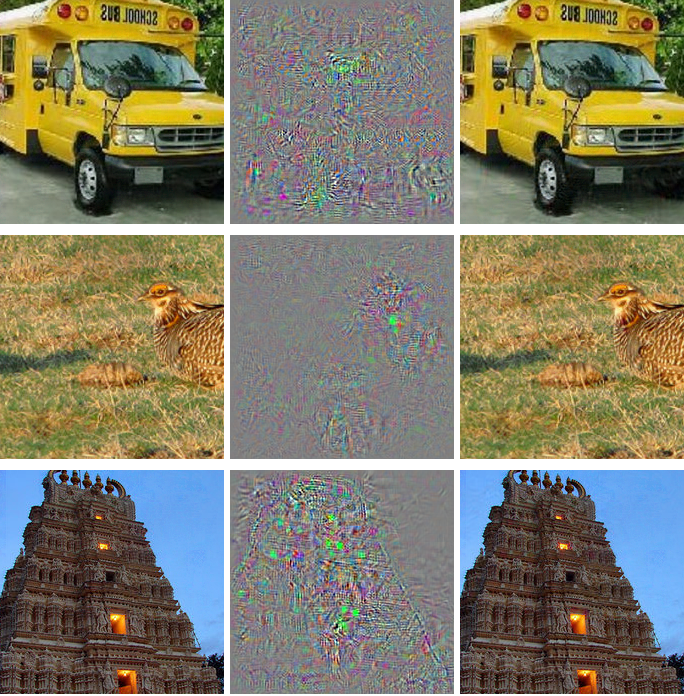
\includegraphics[width=7.3cm]{c1_figures/negative1.png}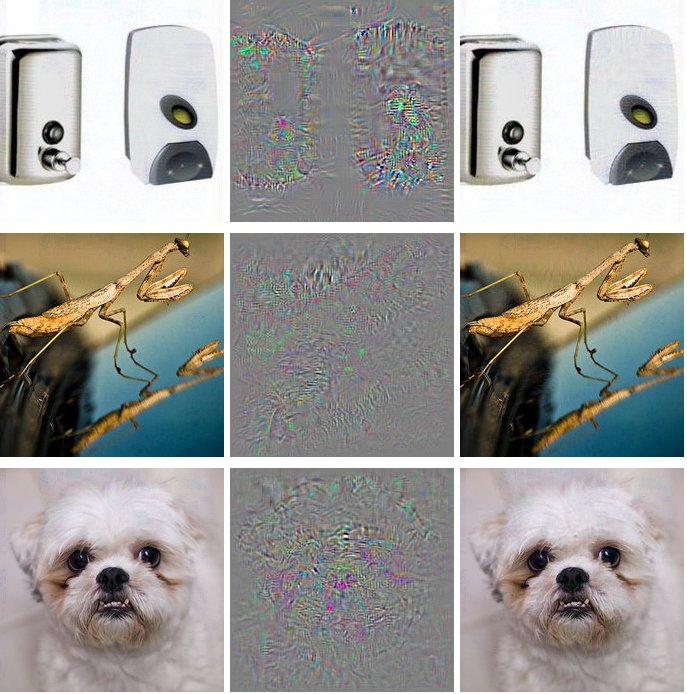
\includegraphics[width=7.3cm]{c1_figures/negative2.png}
    \caption{Natural Images are in columns 1 and 4, Adversarial images are in columns 3 and 6, and the difference between them (magnified by a factor of 10) is in columns 2 and 5. All images in columns 3 and 6 are classified by AlexNet as "Ostrich" \cite{Szegedy2013}}
    \label{fig:my_label}
\end{figure}

\subsubsection{Common Datasets}

The Dataset used above is known as ImageNet -- a large set of labeled images varying in size originally compiled for the ImageNet Large Scale Visual Recognition Challenge (ILSVRC). This dataset and its many subsets has become a standard for image classification and feature identification experiments. In the experiments that follow, ImageNet will be featured alongside the Modified National Institute of Standards and Technology (MNIST) dataset which is a database of hand written digits often used to develop image processing and character recognition systems. This dataset is much lower resolution than ImageNet and is therefore experiments run much more quickly on it and require less complex input/output.  

\subsubsection{L-BFGS minimizing distortion}\label{lbfgs}

Szegedy et al. took advantage of the tools they had on hand for training neural networks to set up a box-constrained optimization problem whose approximated solution generates these targeted misclassifications. 


Let $f : \R^m \to \{1,...,k\}$ be a classifier and assume $f$ has an associated continuous loss function denoted by loss$_f : \R^m \times \{1,...,k\} \to \R^+$ and $l$ a target adversarial . \\
\textbf{ Minimize} $\Norm{r}_2$ subject to:
\begin{enumerate}[1.]
\item $f(x + r) = l$
\item $x + r \in [0,1]^m$
\end{enumerate}

The solution is approximated with L-BFGS (see Appendix \ref{appa}) as implemented in Pytorch or Keras. This technique yields examples that are close to their original counterparts in the $L^2$ sense.  \\

%Find the minimum $c > 0$ for which the minimizer $r$ of the following satisfies $f(x+r) = l$\\

%minimize $c|r| + $loss$_f(x+r,l)$ subject to $x + r \in [0,1]^m$.

\paragraph{L-BFGS: Mnist}
The following examples are prepared by implementing the above technique via pytorch on images from the Mnist dataset with FC200-200-10, a neural network with 2 hidden layers with 200 nodes each:
\begin{figure}[H]
\label{lbfgsa}
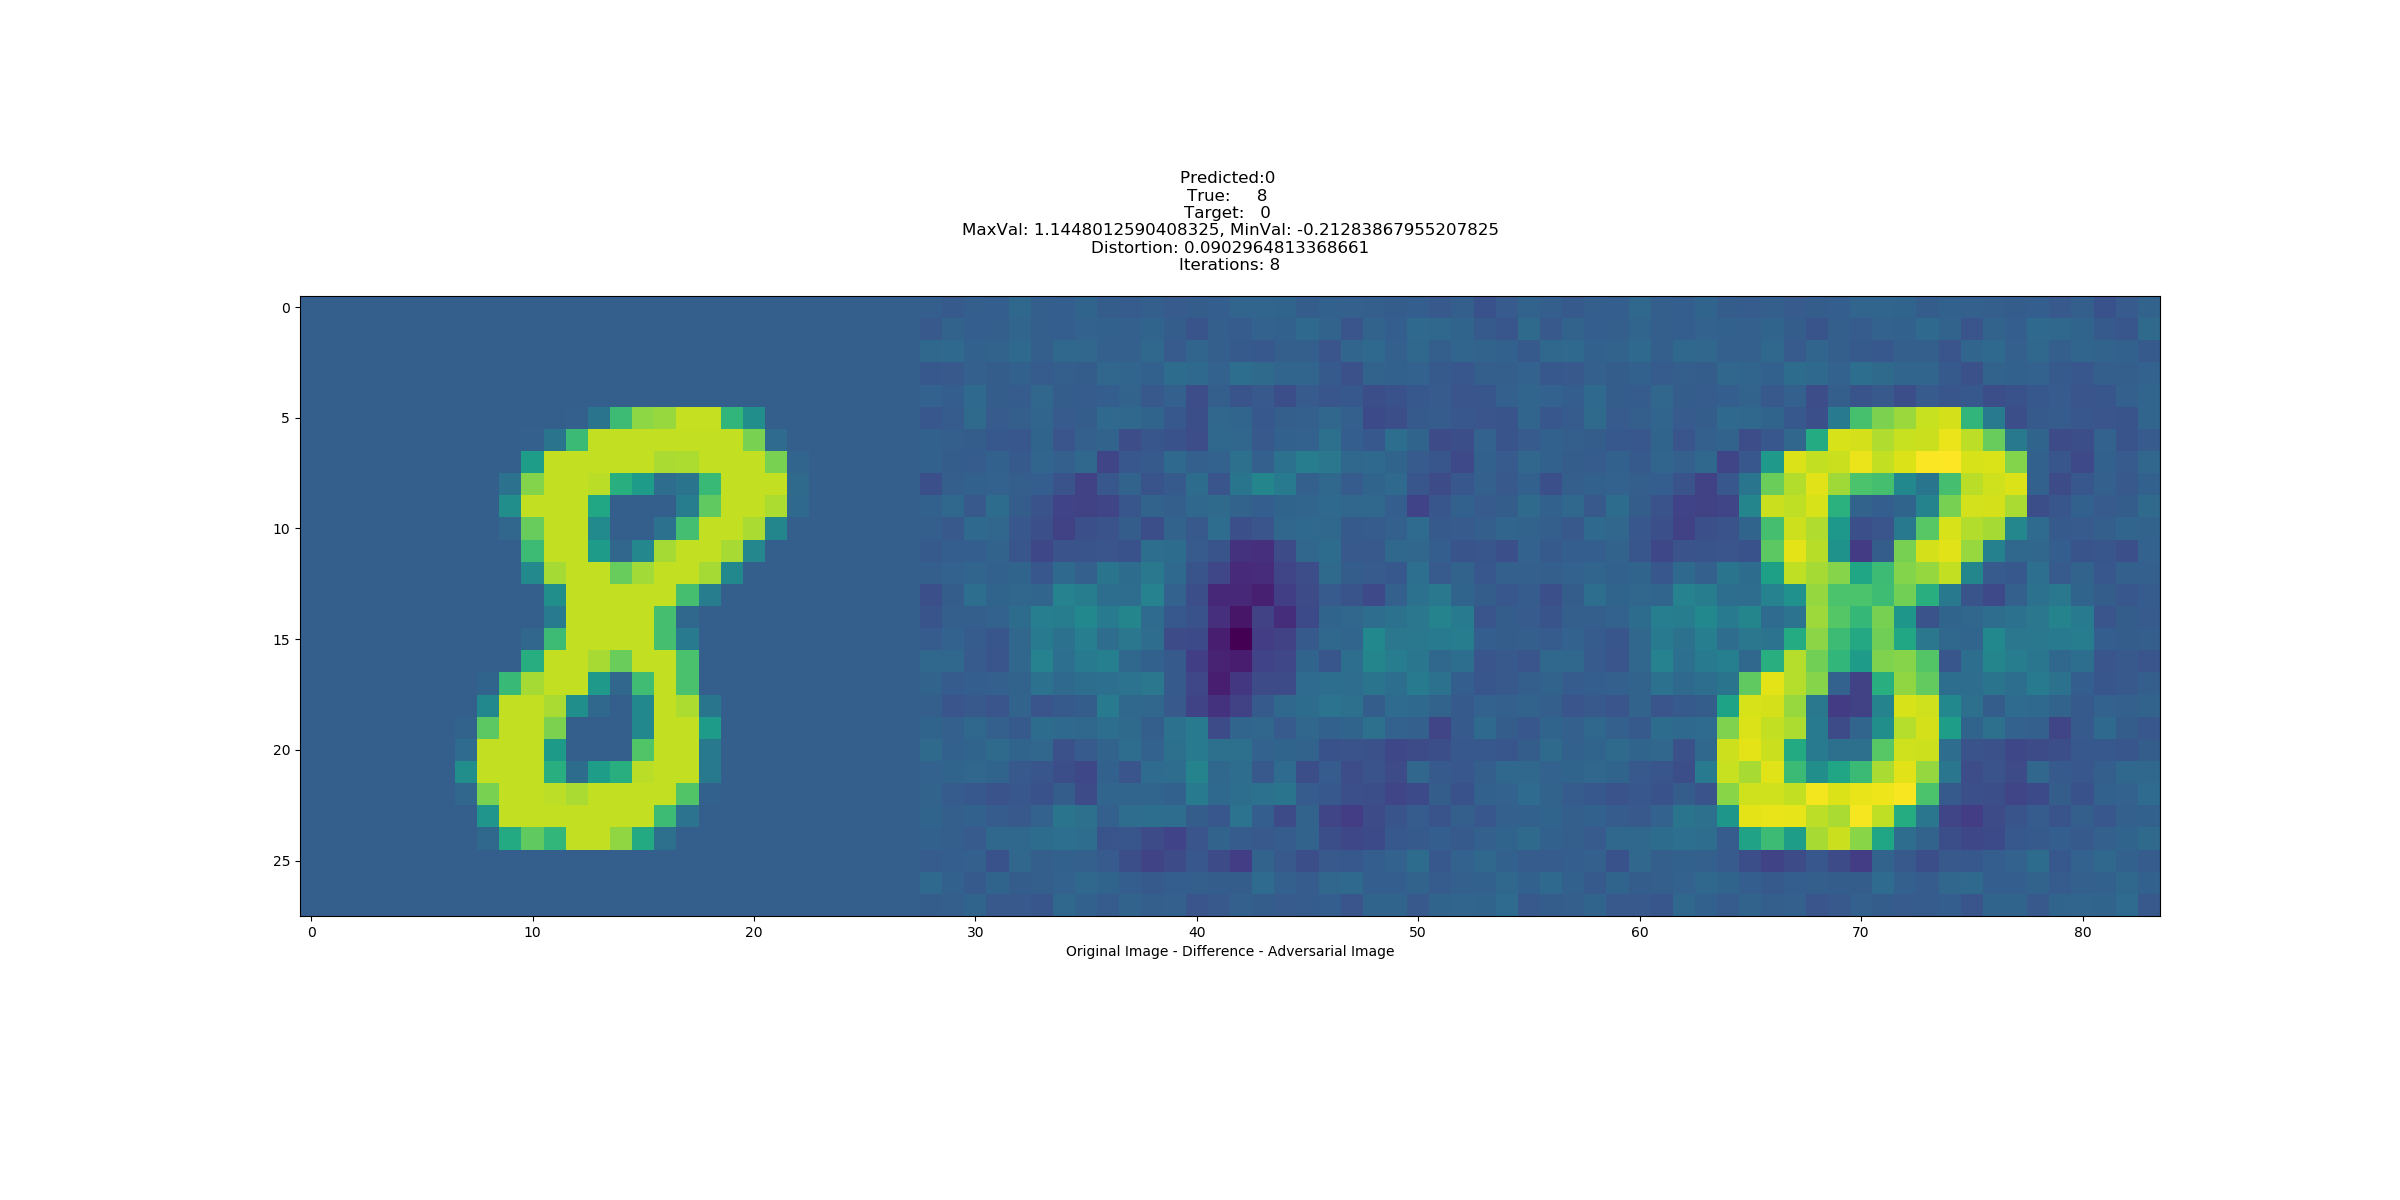
\includegraphics[trim=200 185 100 200, clip, width=7cm]{c1_figures/FC200-200-10-2448-O8-A0-attack_summary.png}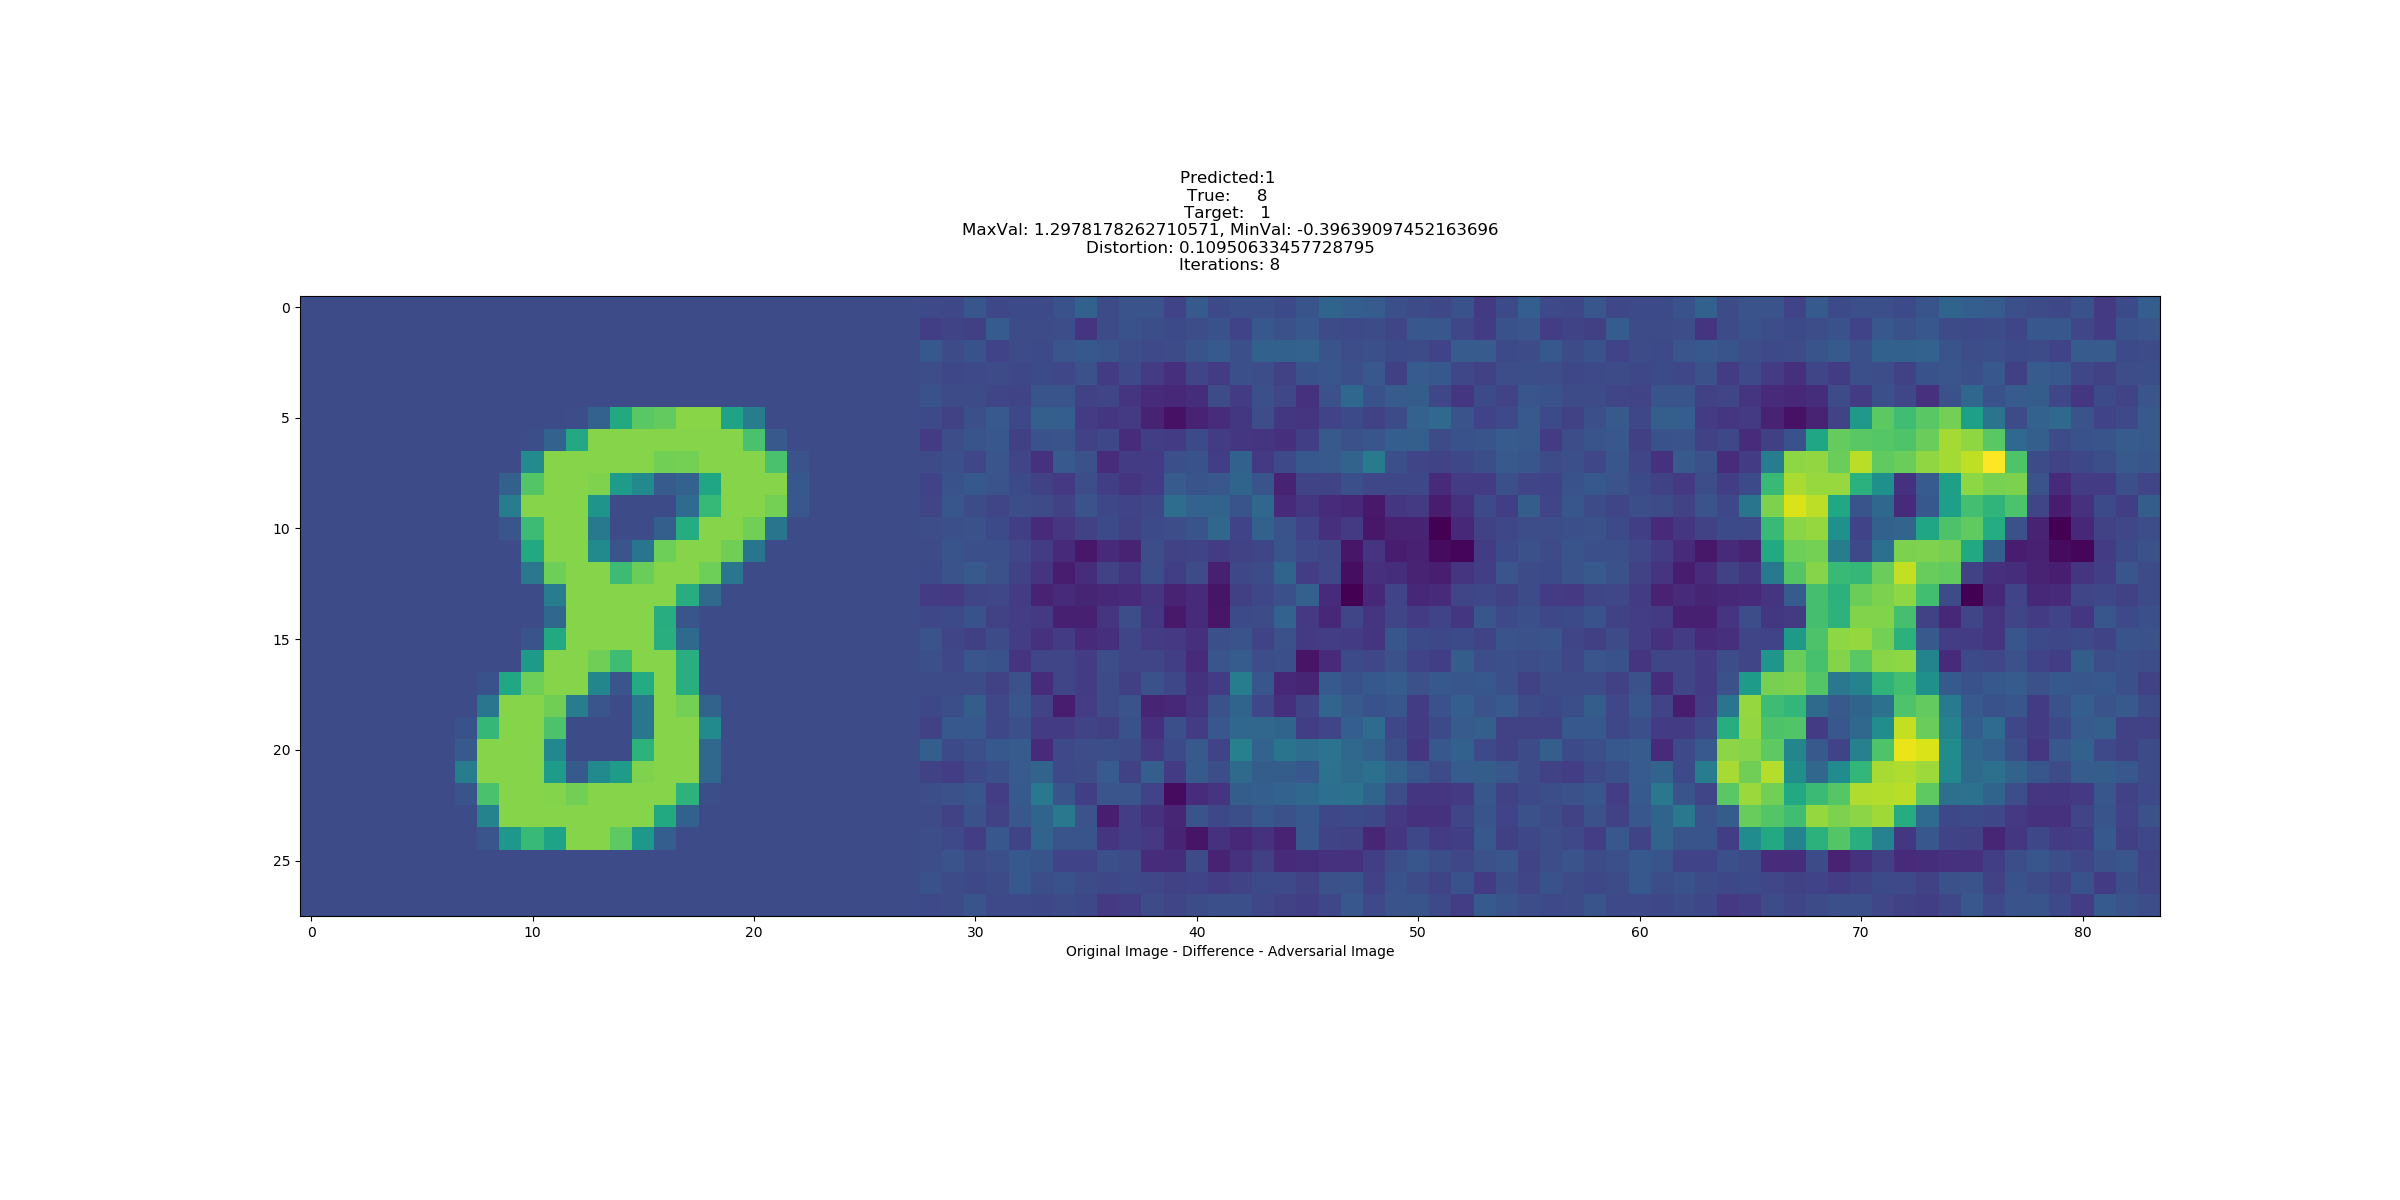
\includegraphics[trim=200 185 100 200, clip,width=7cm]{c1_figures/FC200-200-10-2448-O8-A1-attack_summary.png}
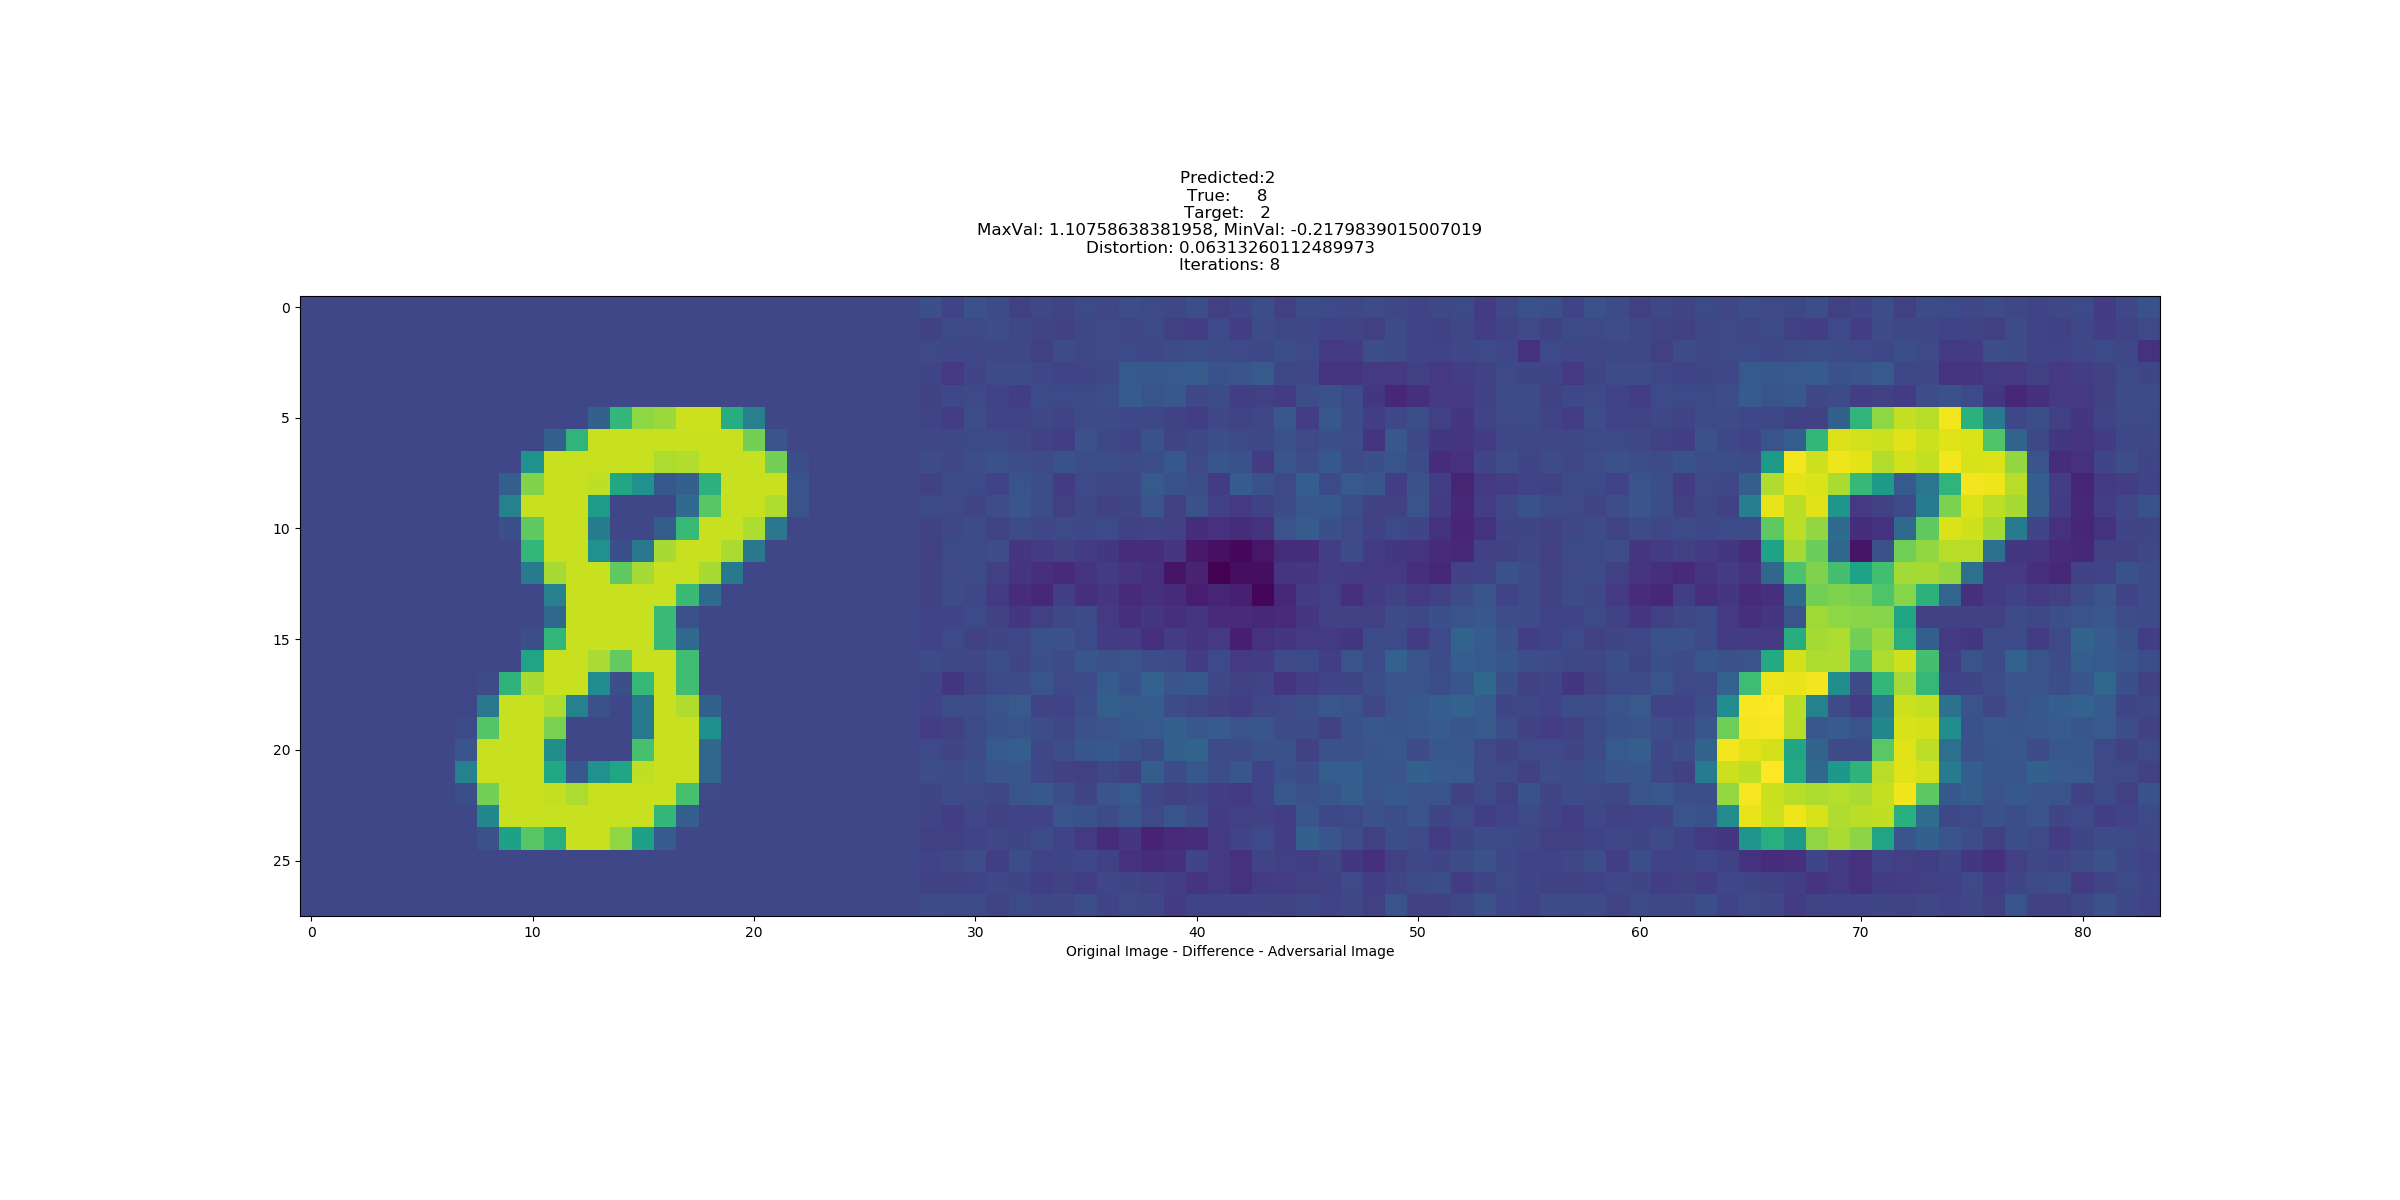
\includegraphics[trim=200 185 100 200, clip,width=7cm]{c1_figures/FC200-200-10-2448-O8-A2-attack_summary.png}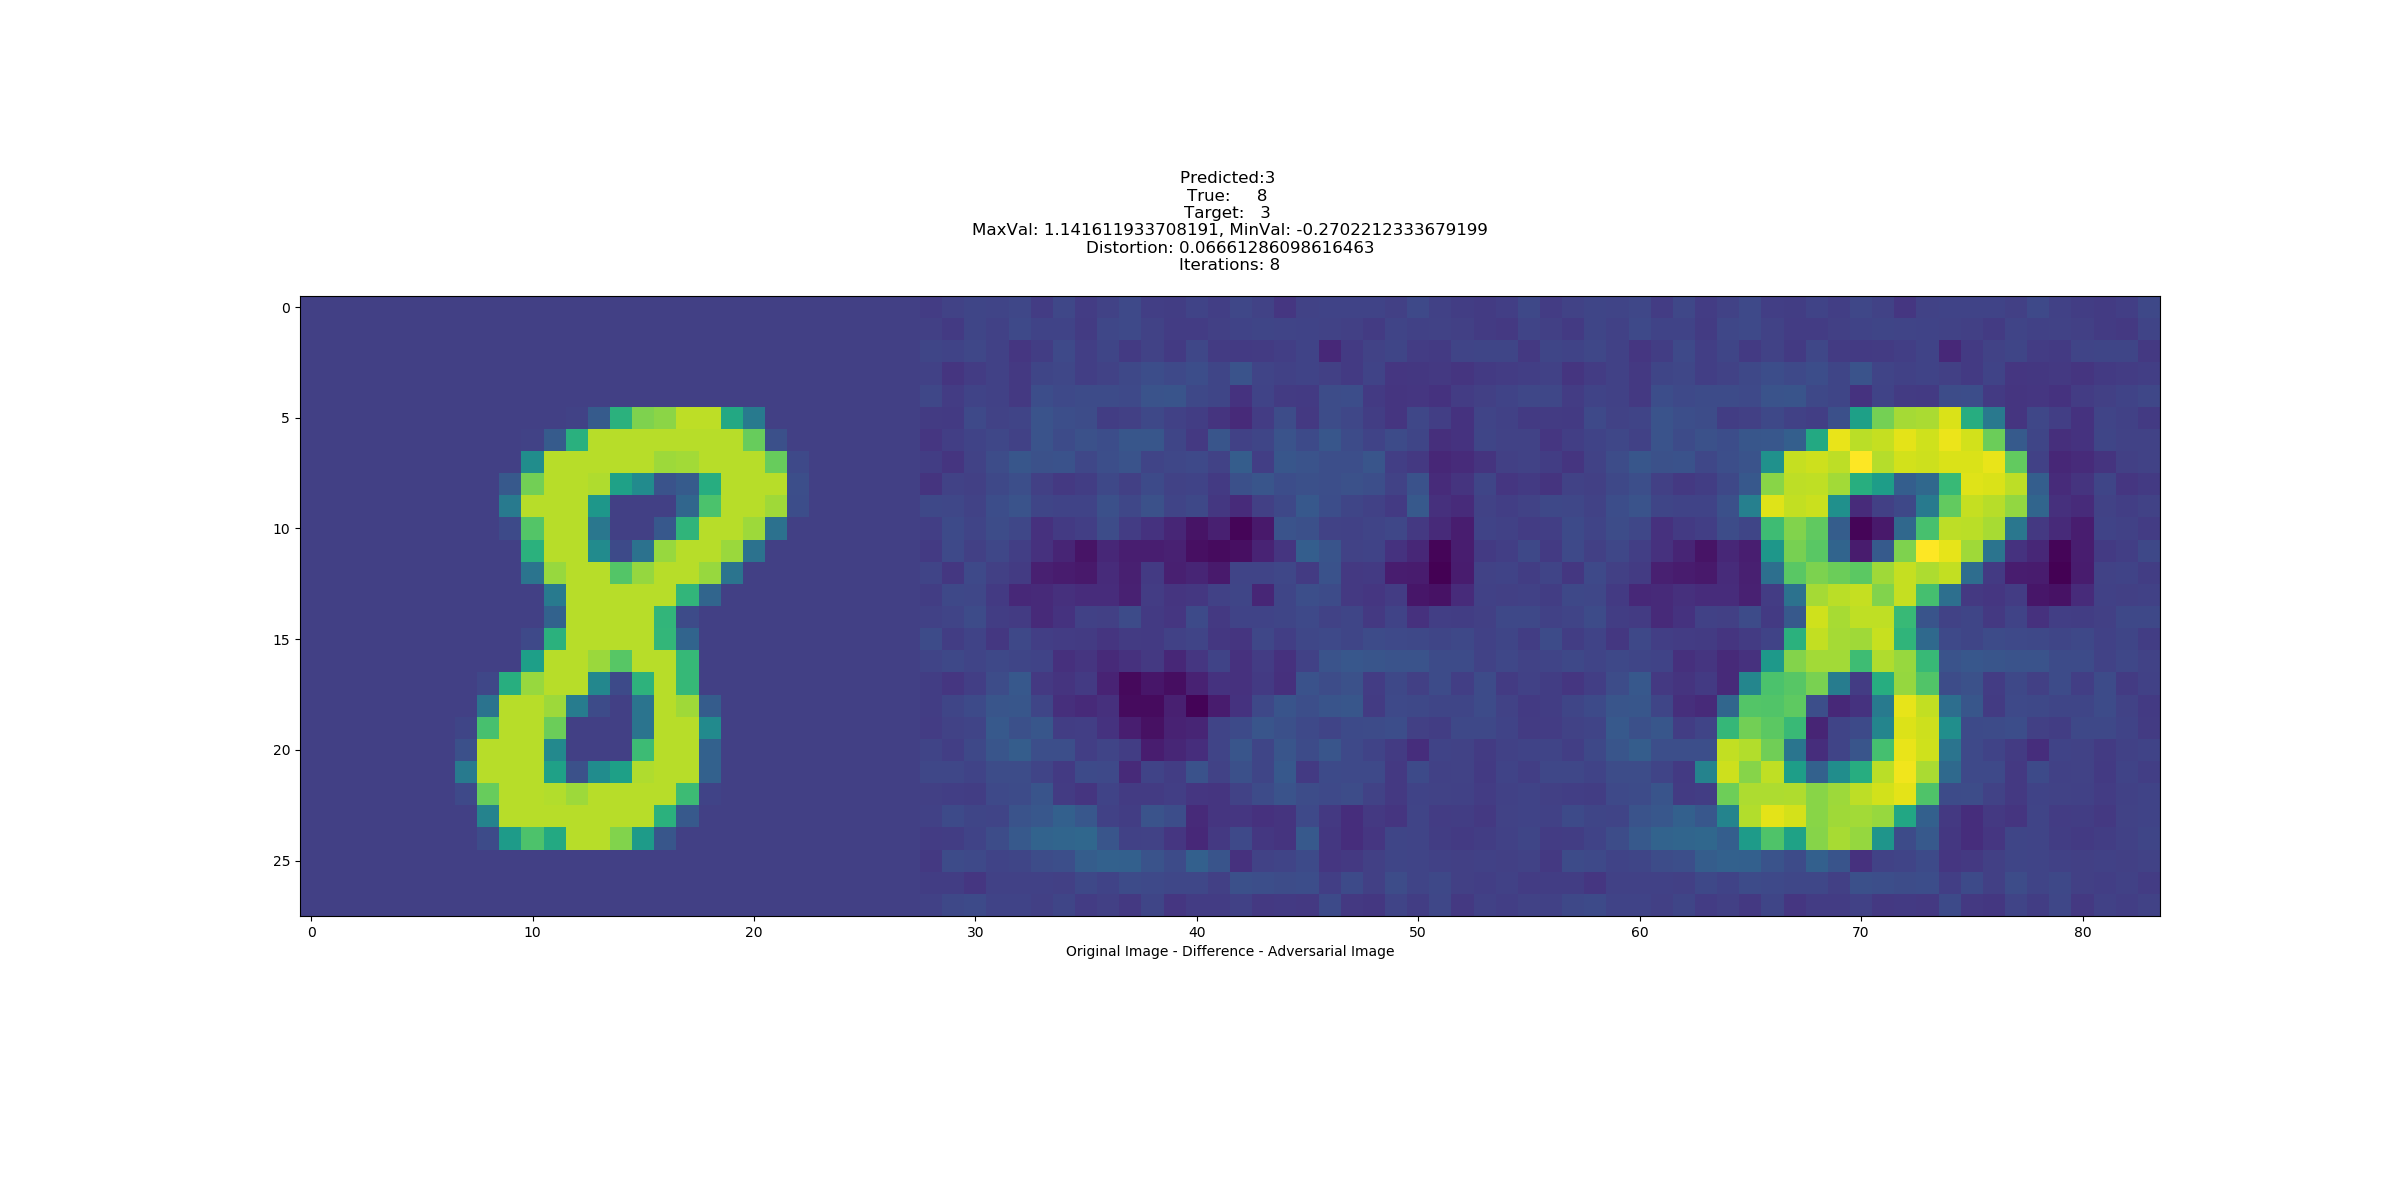
\includegraphics[trim=200 185 100 200, clip,width=7cm]{c1_figures/FC200-200-10-2448-O8-A3-attack_summary.png}
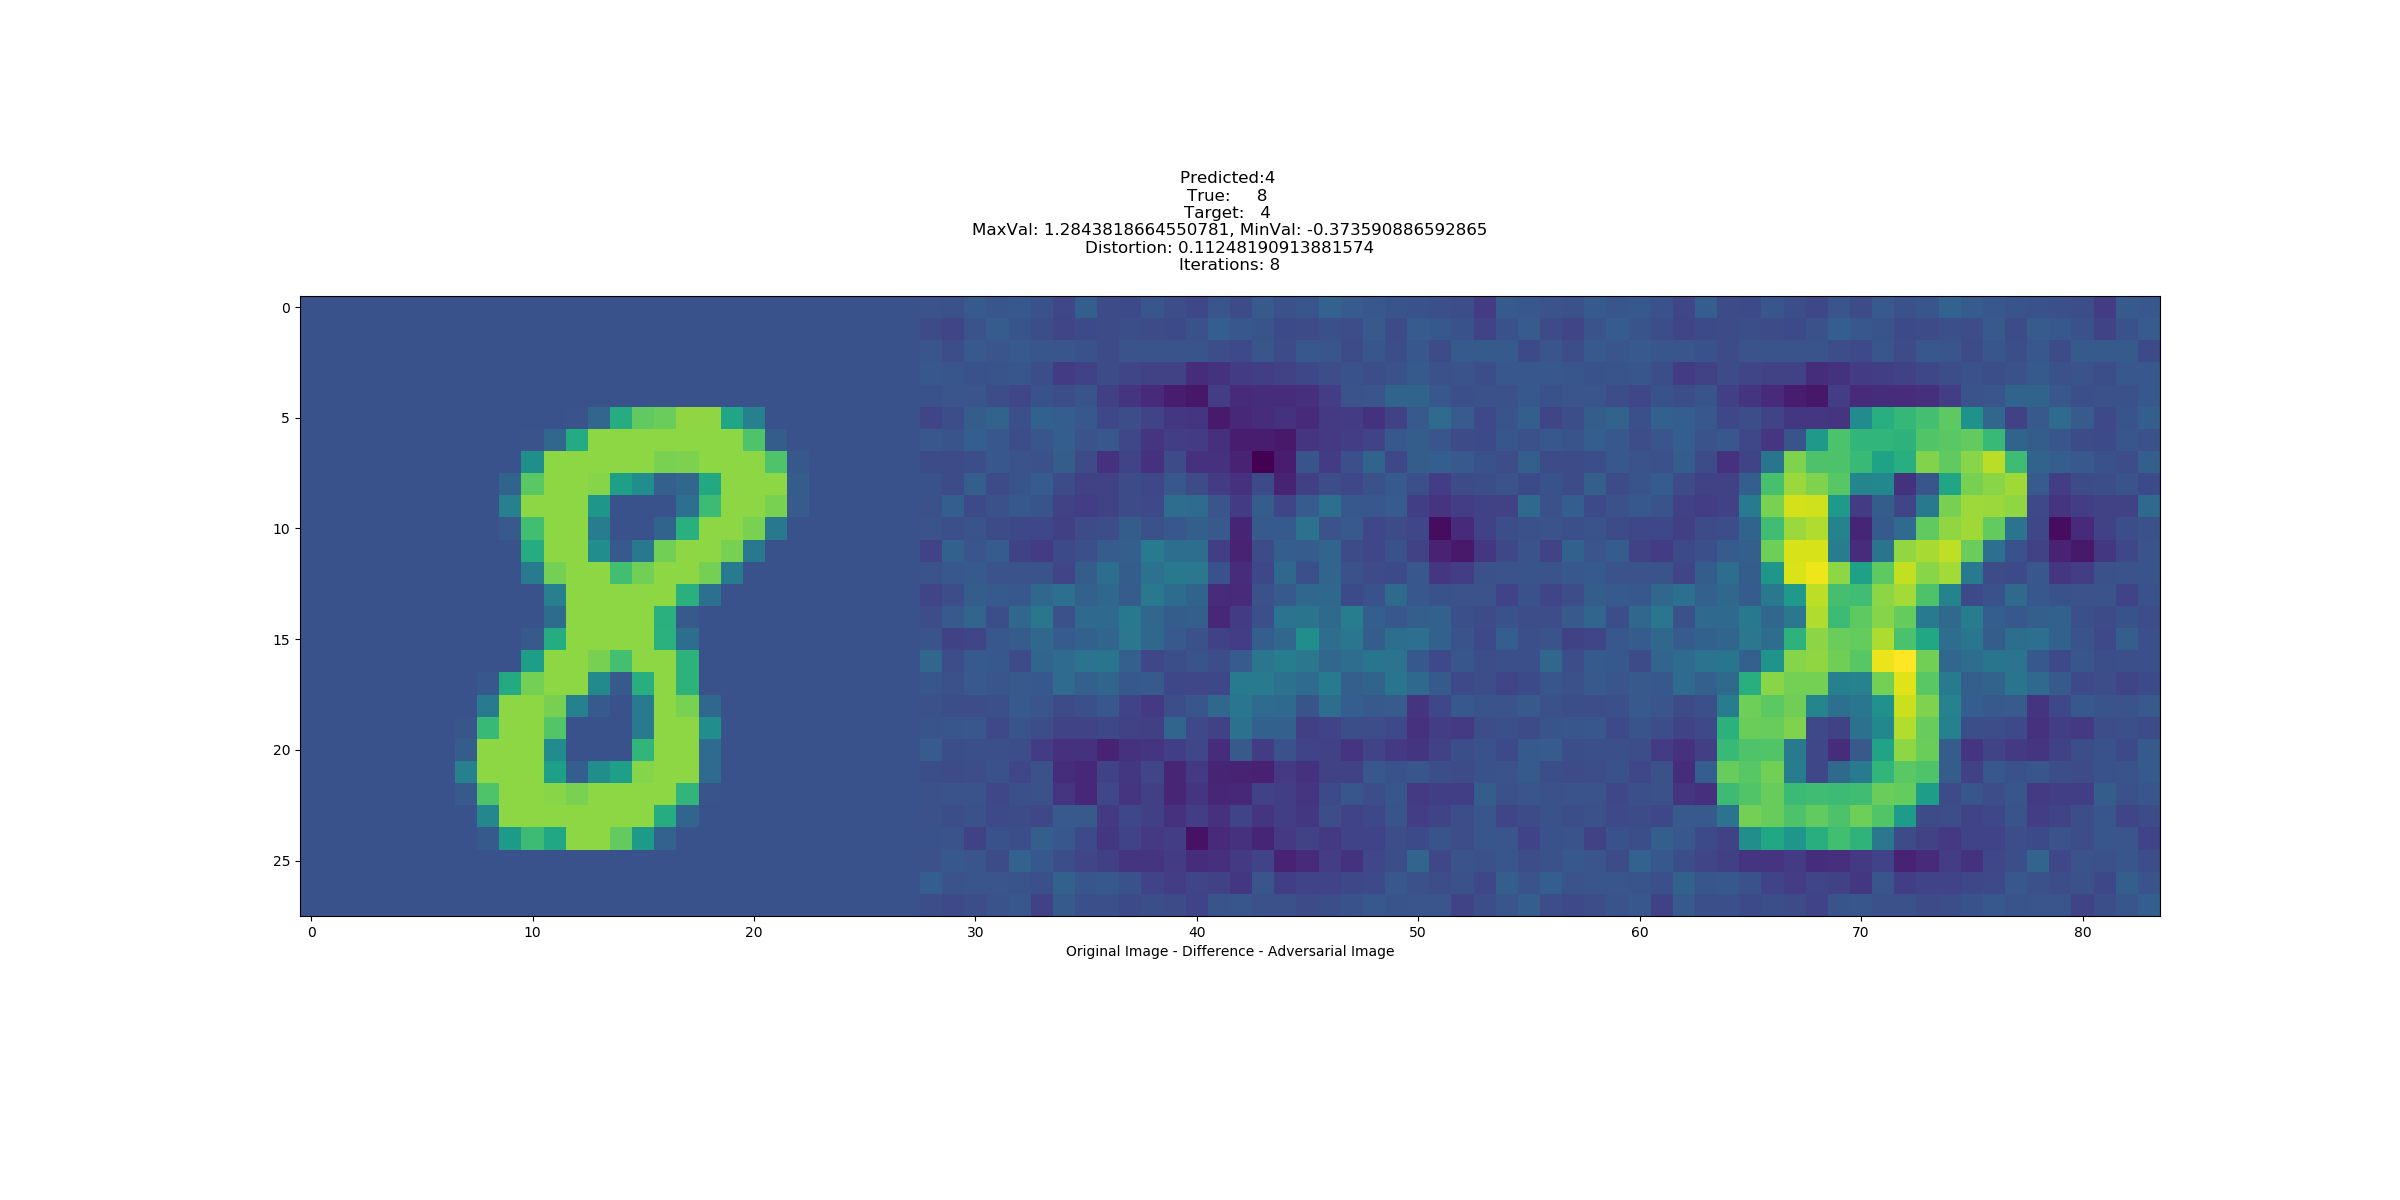
\includegraphics[trim=200 185 100 200, clip,width=7cm]{c1_figures/FC200-200-10-2448-O8-A4-attack_summary.png}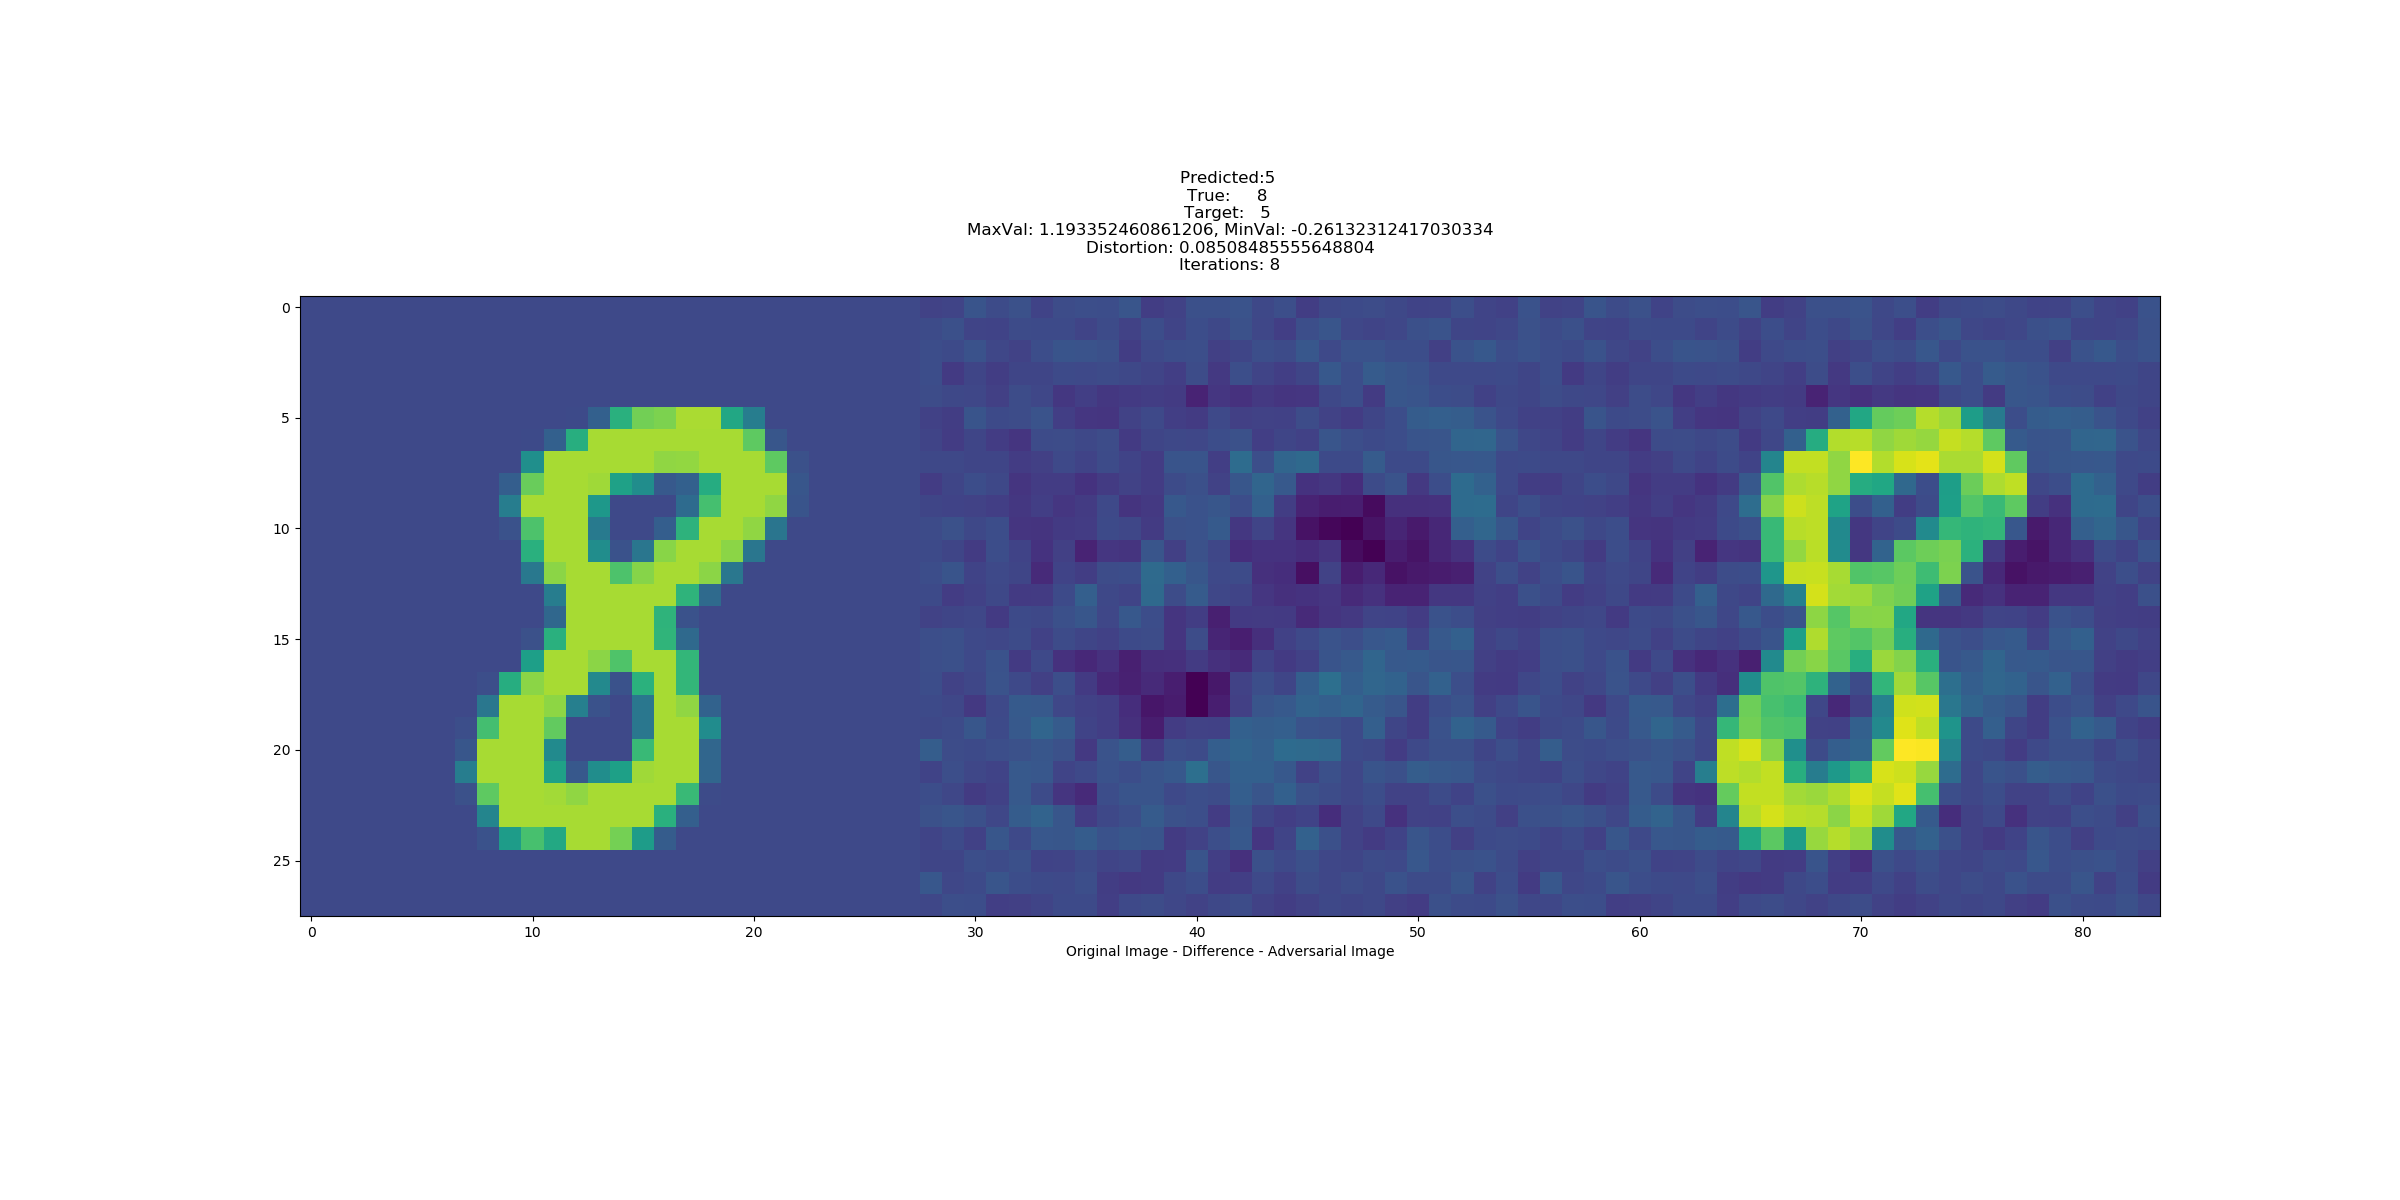
\includegraphics[trim=200 185 100 200, clip,width=7cm]{c1_figures/FC200-200-10-2448-O8-A5-attack_summary.png}
\caption{Original images on the left, Perturbation is in the middle, Adversarial Image (total of Original with Perturbation) is on the right. Column 1 shows an original 8 being perturbed to adversarial classes 0, 2, and 4. Column 2 shows adversarial classes 1, 3, and 5}
\end{figure}
Borrowing a metric from Szegedy et al to compare the magnitude of these distortions, we will define
\begin{definition}{Distortion is the $L^2$ norm of the difference between an original image and a perturbed image, divided by the square root of the number of pixels in the image: }
\[\sqrt{\dfrac{\sum_i \hat (x_i - x_i)^2}{n}}\]
\end{definition}
Distortion is $L^2$ magnitude normalized by the square-root of the number of dimensions so that values can be compared for modeling problems with differing numbers of dimensions. 

The 900 examples generated for the network above had an average distortion of 0.089 with the following distribution of distortions, given in figure 3.

\begin{figure}[H]
\label{lbfgsh}
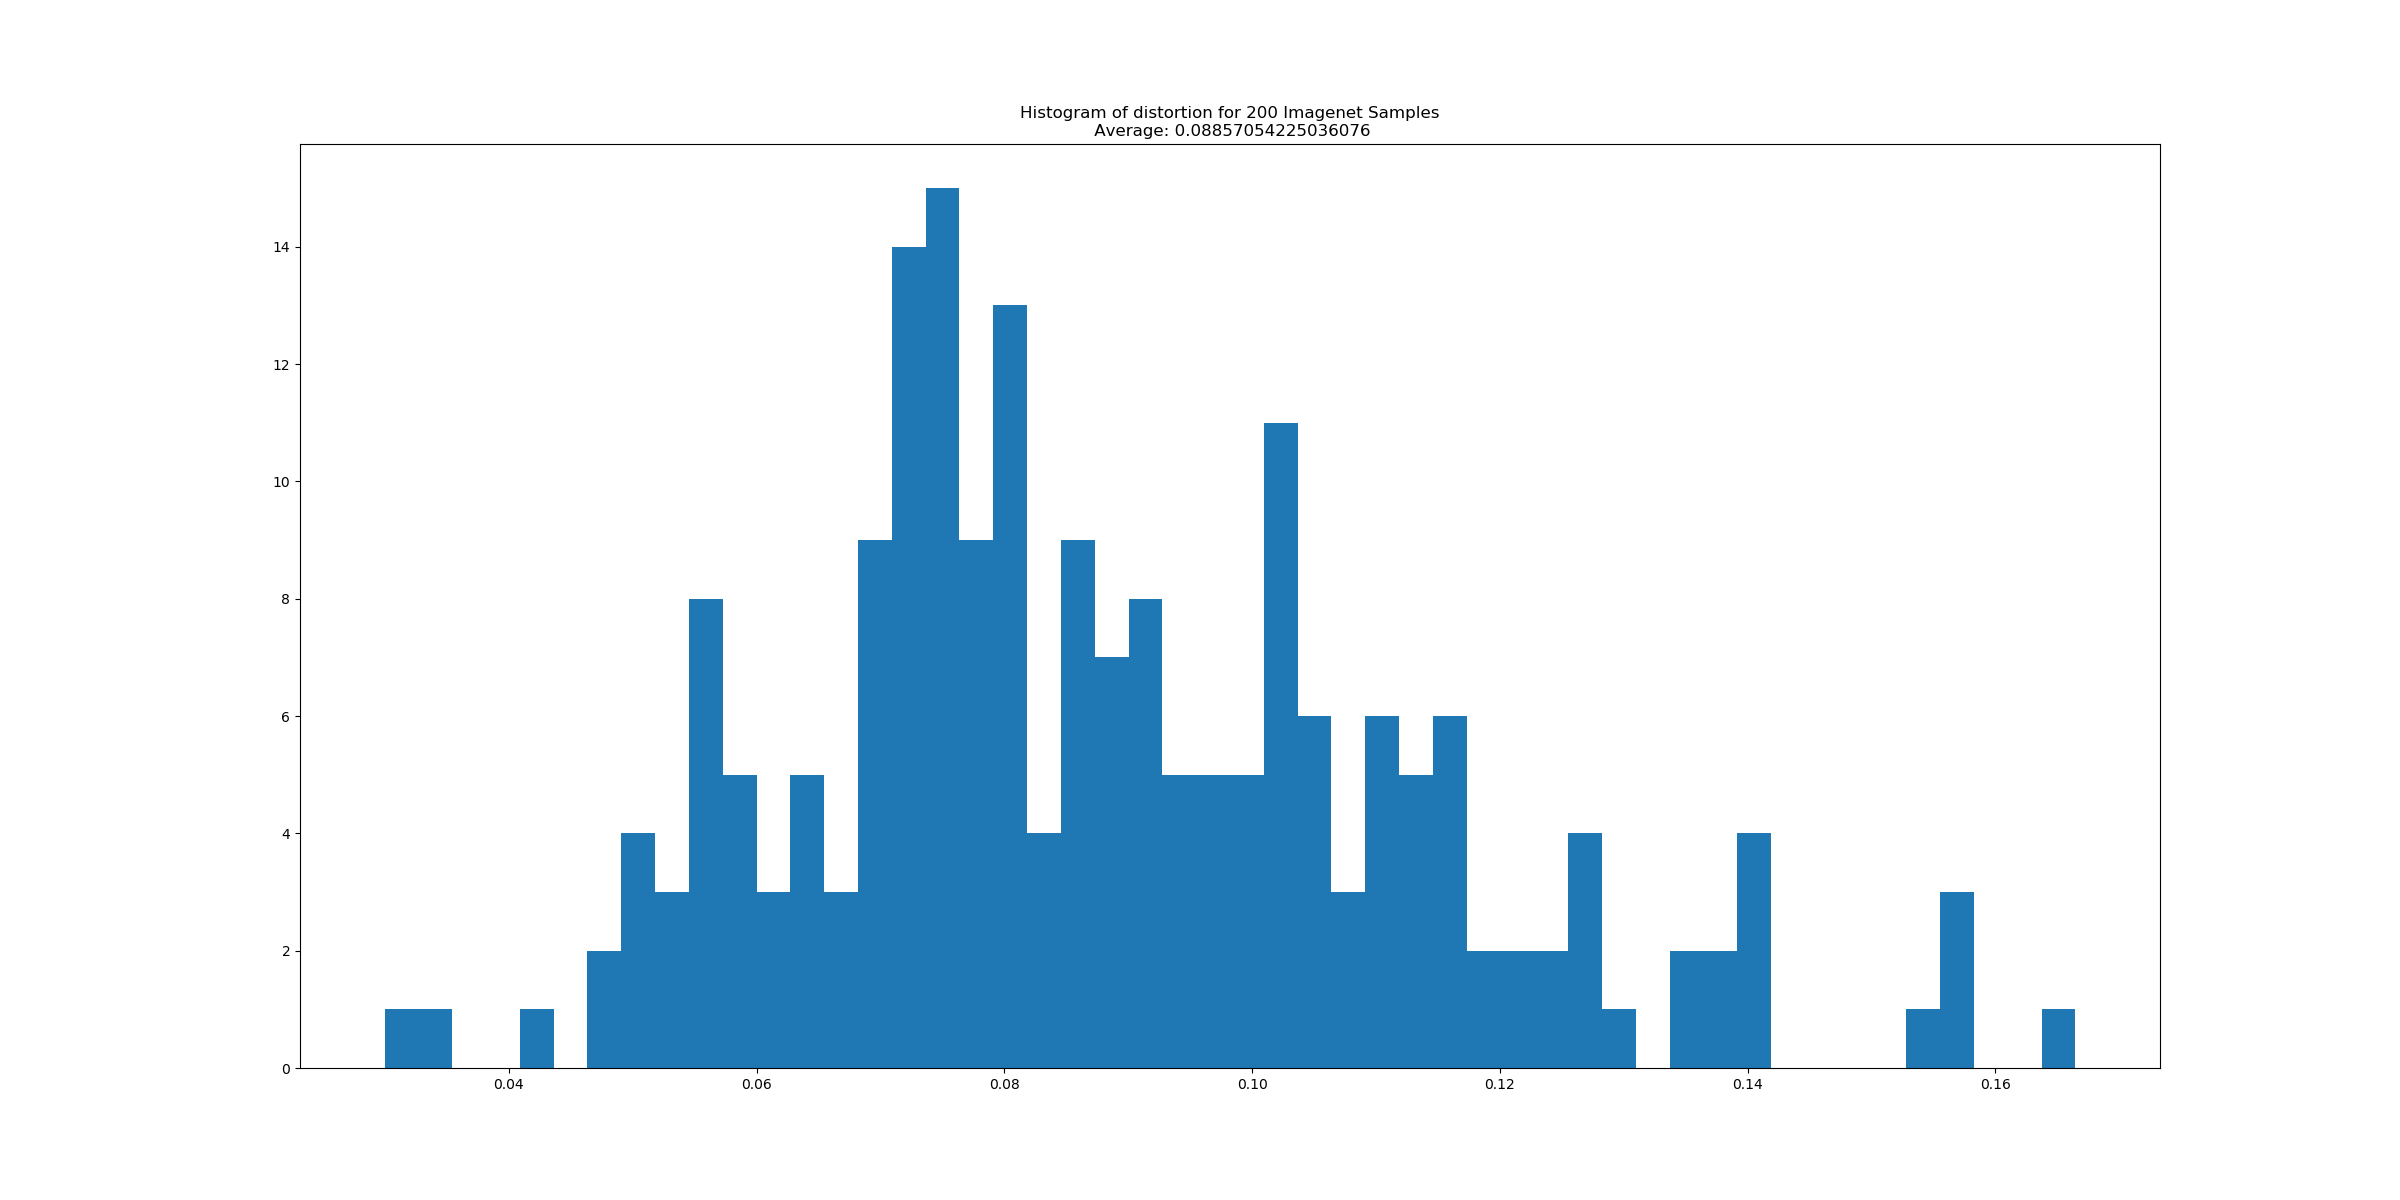
\includegraphics[trim=200 80 100 100, clip, width=16cm]{c1_figures/FC200-200-10-distortion_hist.png}
\caption{A histogram of the distortion measured for each of 900 adversarial examples generated using L-BFGS against the FC-200-200-10 network on Mnist. Mean distortion is 0.089.}
\end{figure}

\paragraph{L-BFGS: ImageNet}
\label{lbfgs-s}
We also tried to replicate \cite{Szegedy2013}'s results on ImageNet. Attacking VGG16, a well known model from the ILSVRC-2014 competition \cite{simonyan2014very}, on ImageNet images with the same technique generates the examples in figure 4: 

\begin{figure}[H]
\label{lbfgsis}
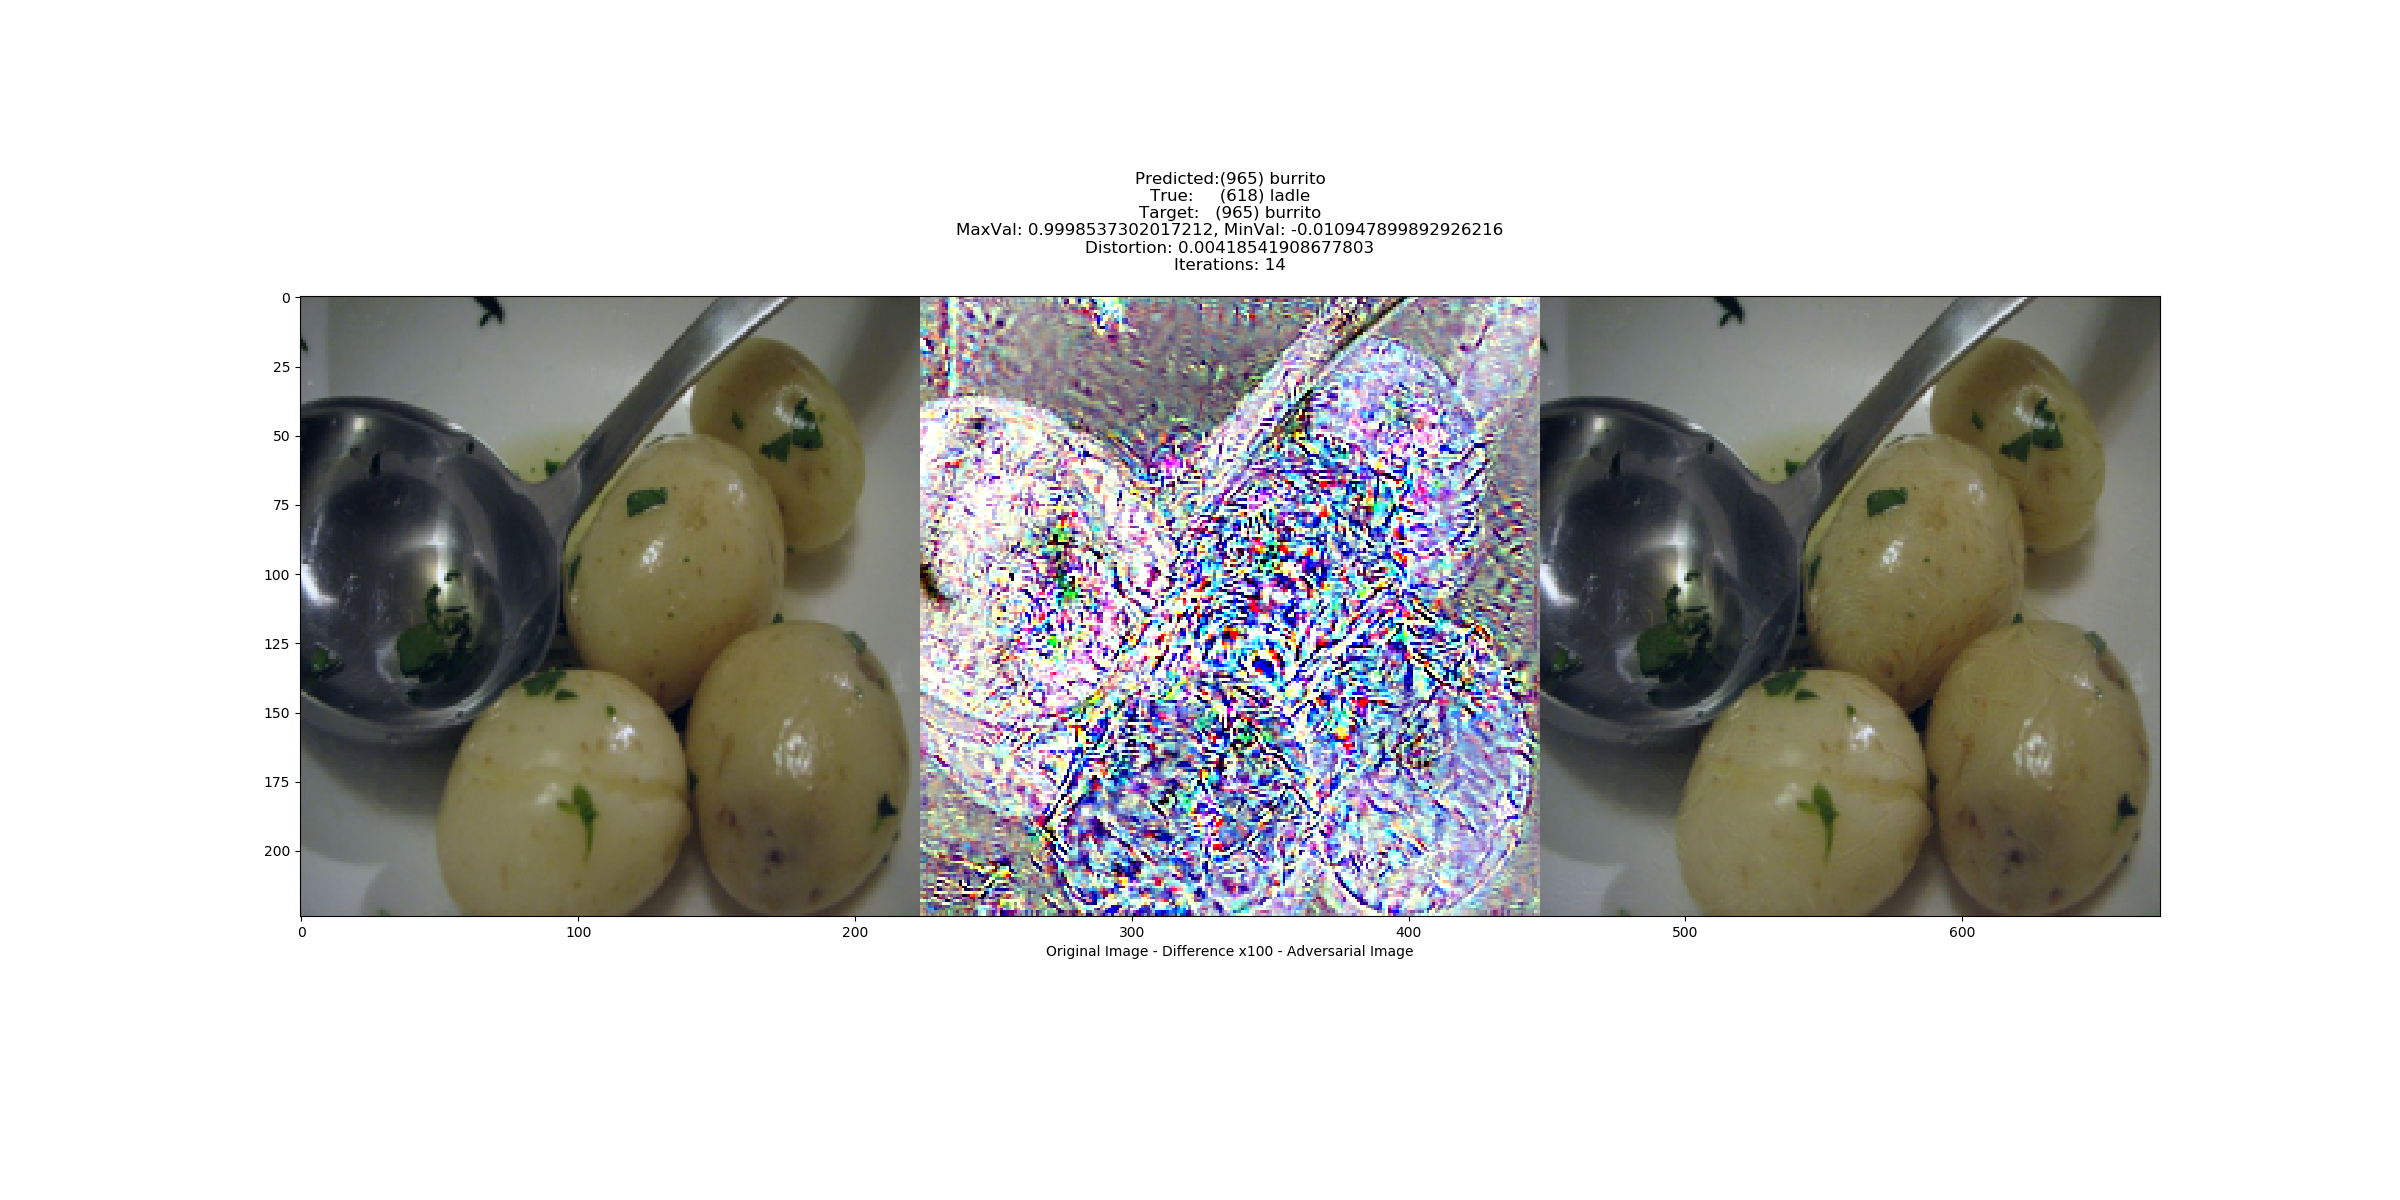
\includegraphics[trim=200 185 100 200, clip, width=8cm]{c1_figures/vgg16-ILSVRC2012_val_00039098-O722-A965-attack_summary.png}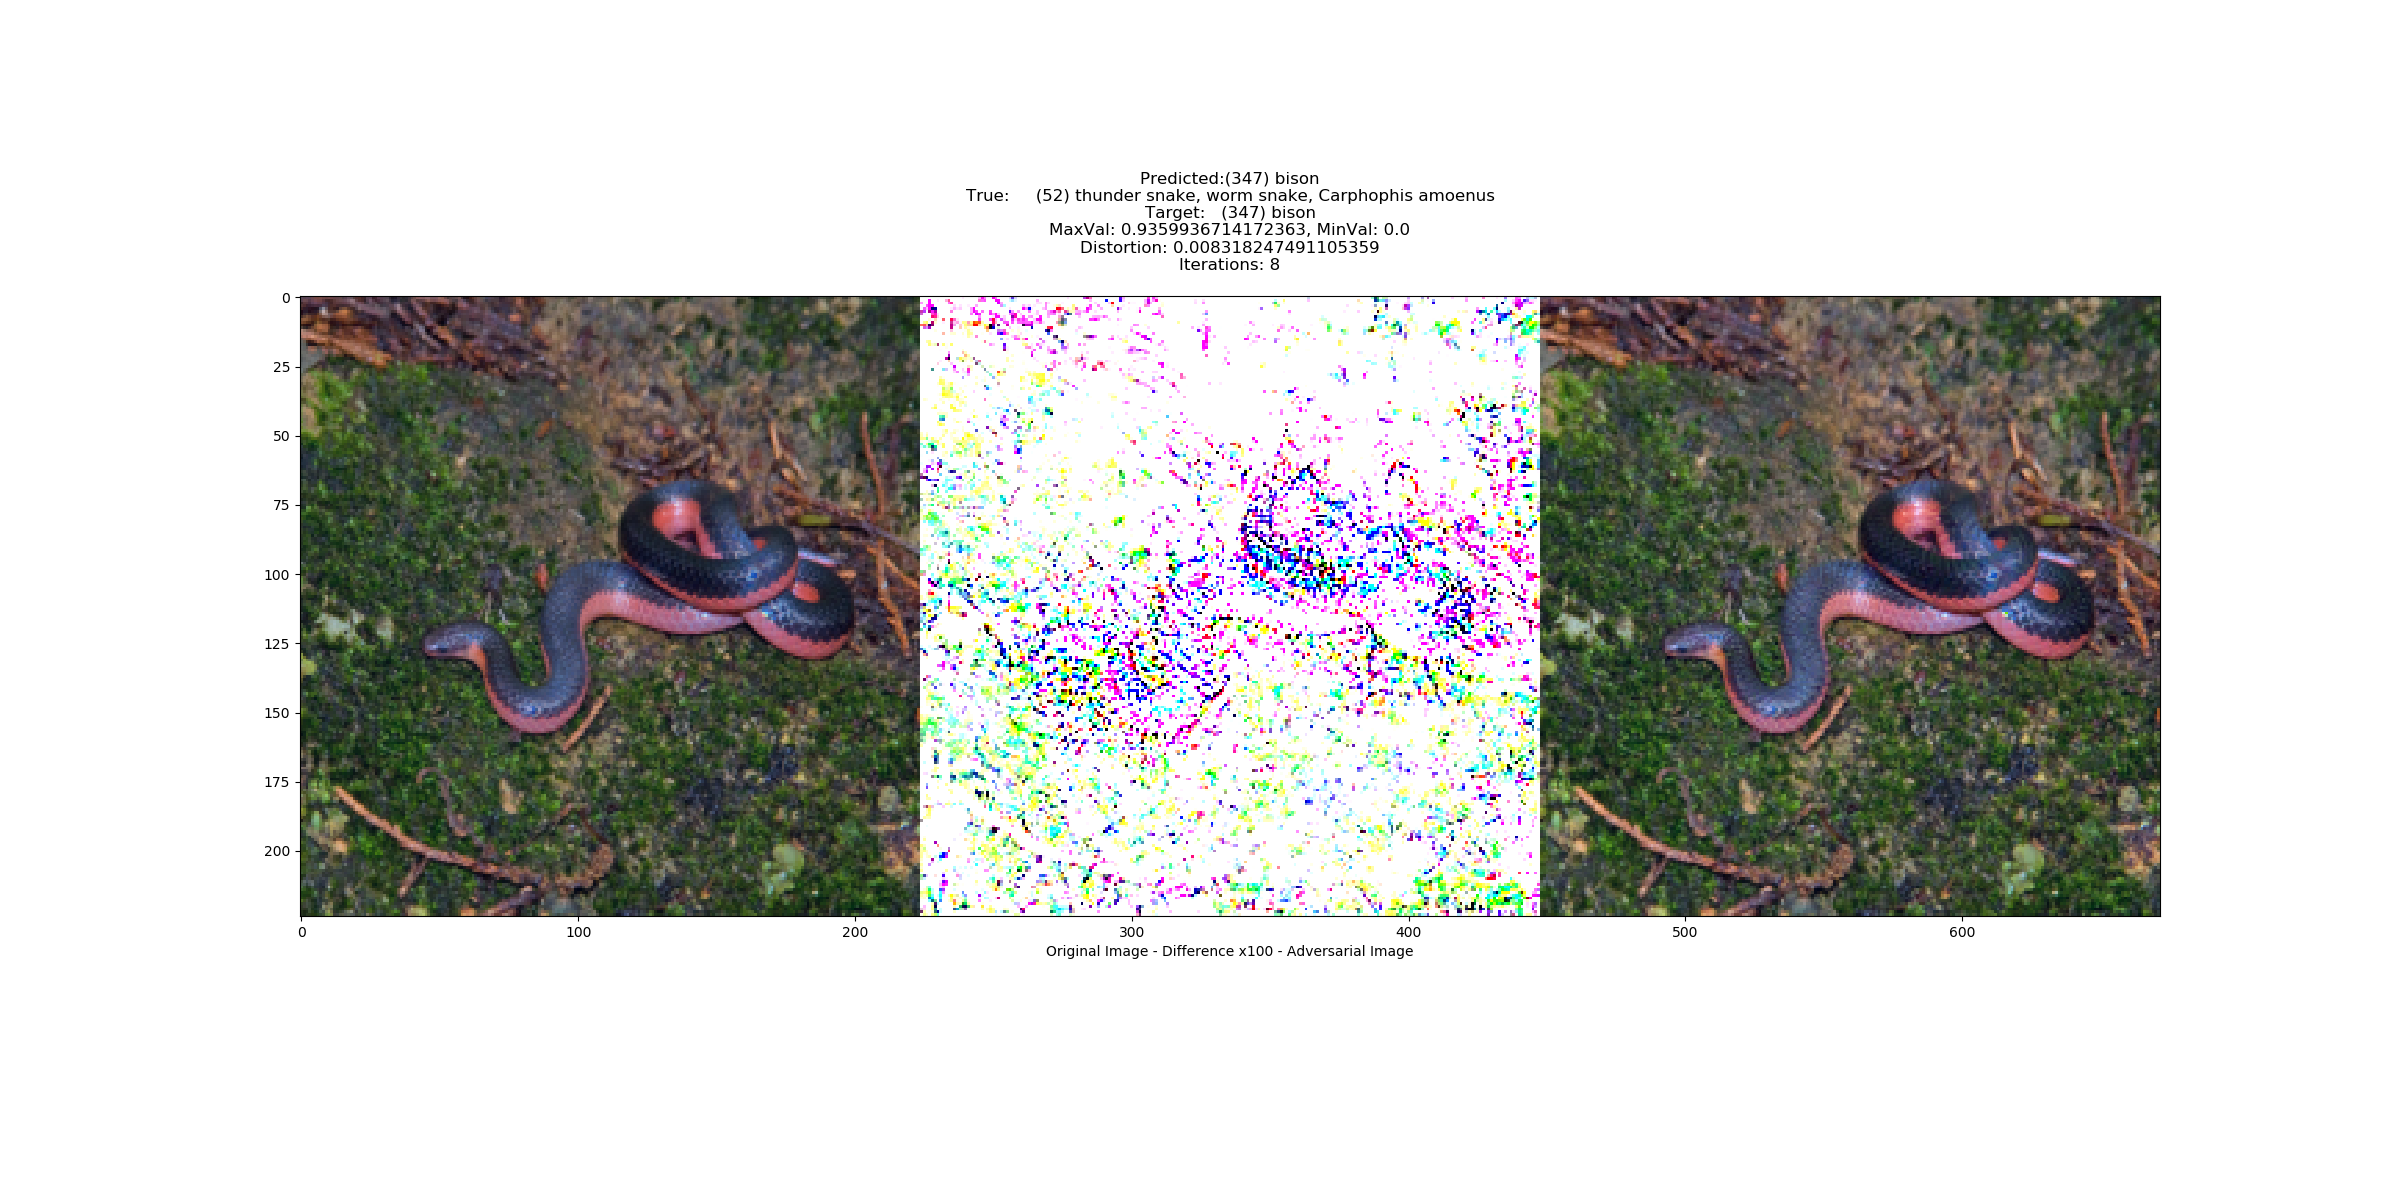
\includegraphics[trim=200 185 100 200, clip, width=8cm]{c1_figures/vgg16-ILSVRC2012_val_00027142-O52-A347-attack_summary.png}
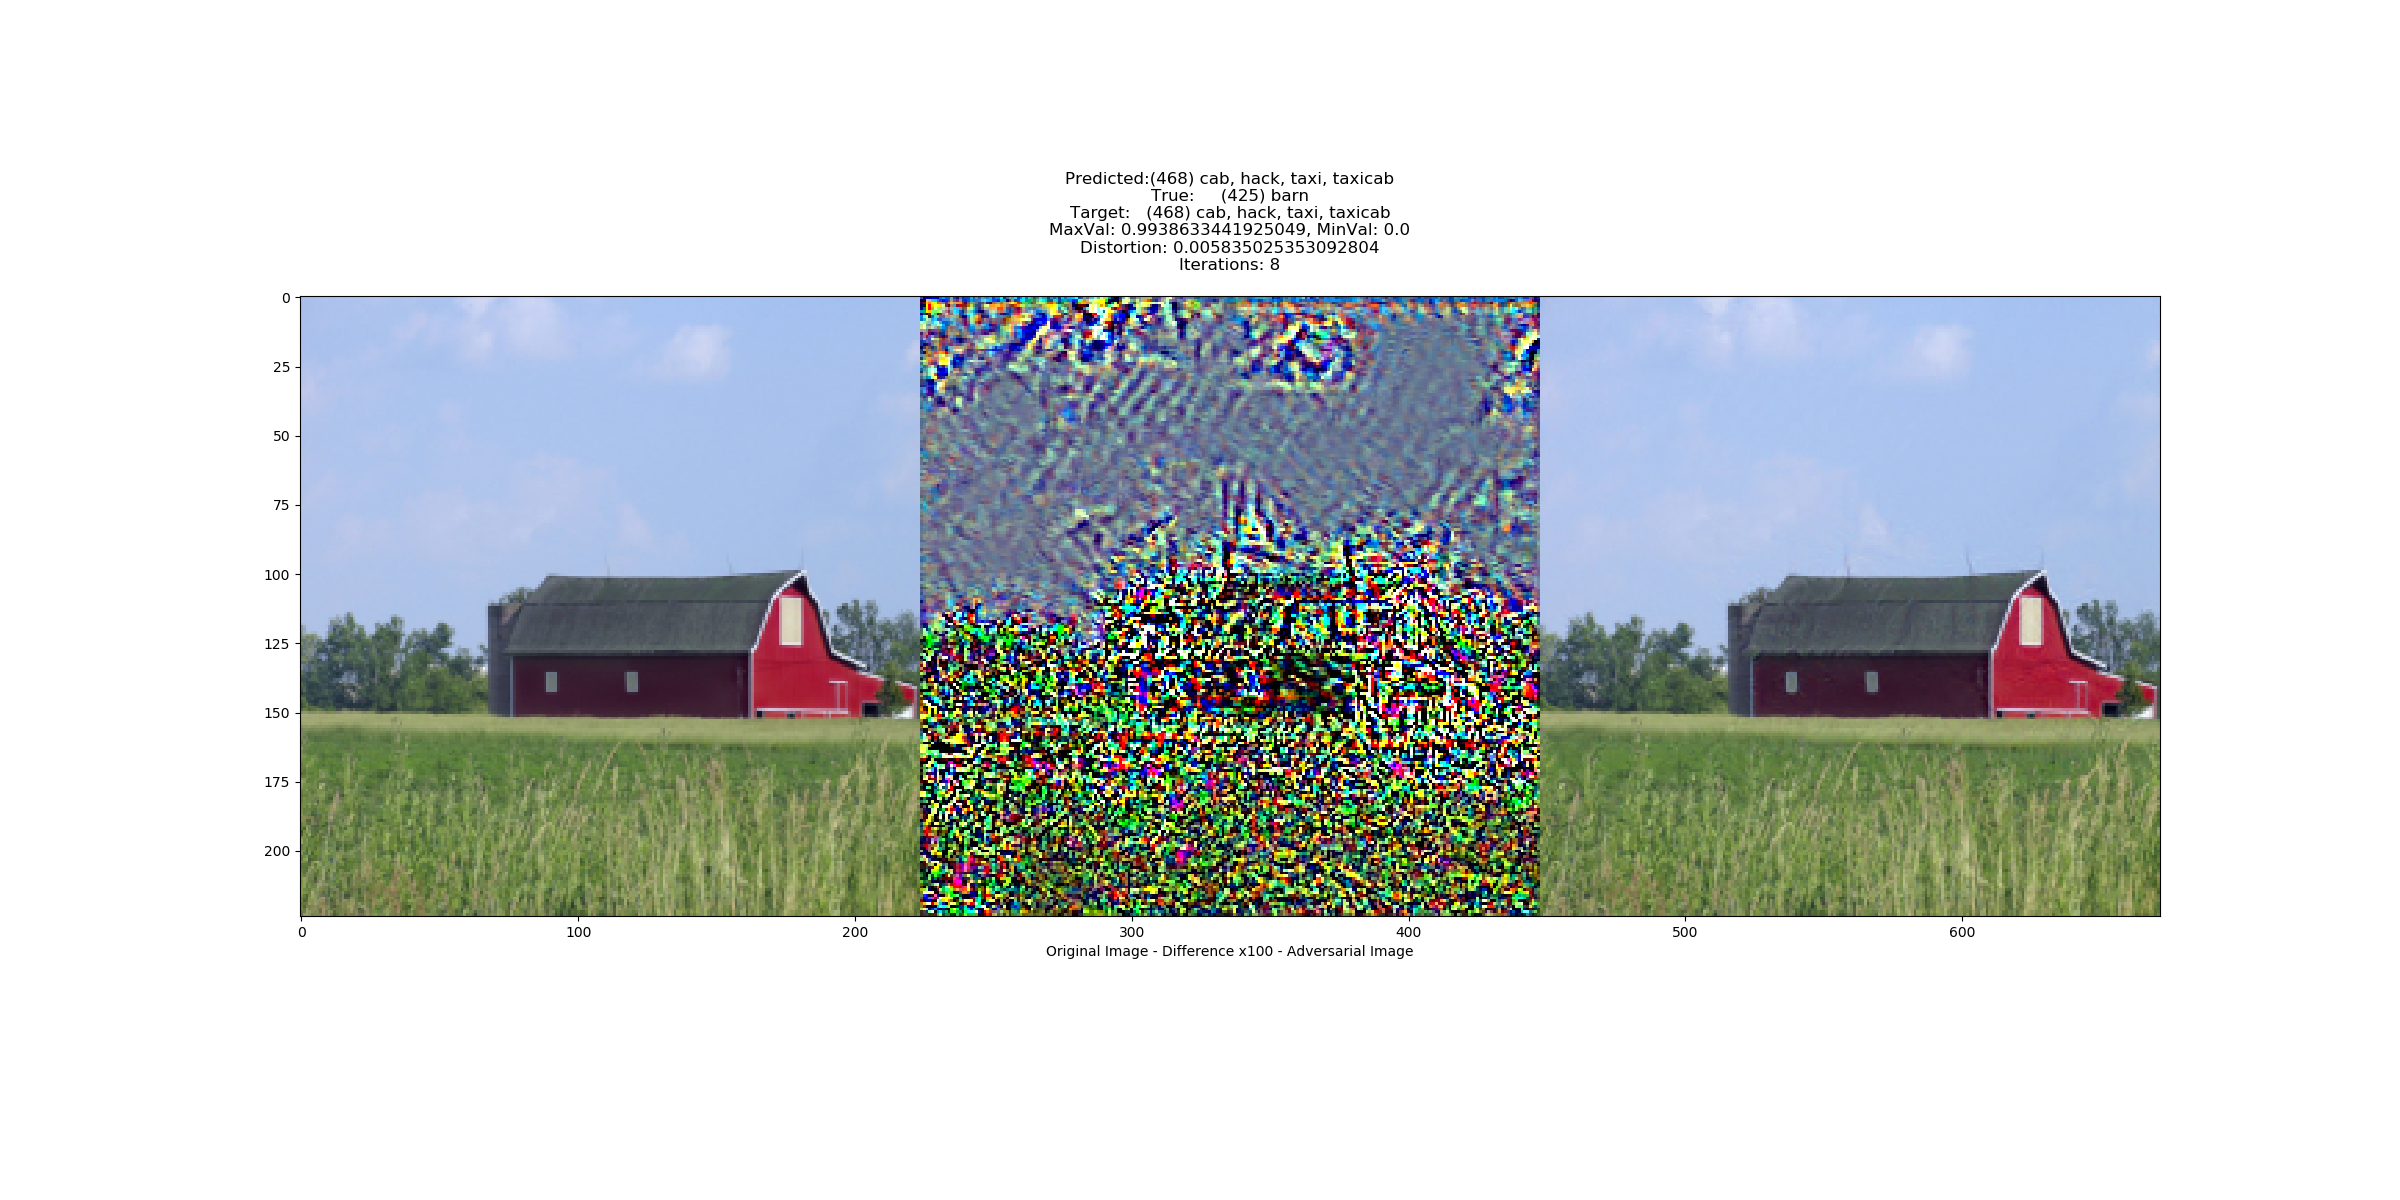
\includegraphics[trim=200 185 100 200, clip, width=8cm]{c1_figures/vgg16-ILSVRC2012_val_00029901-O425-A468-attack_summary.png}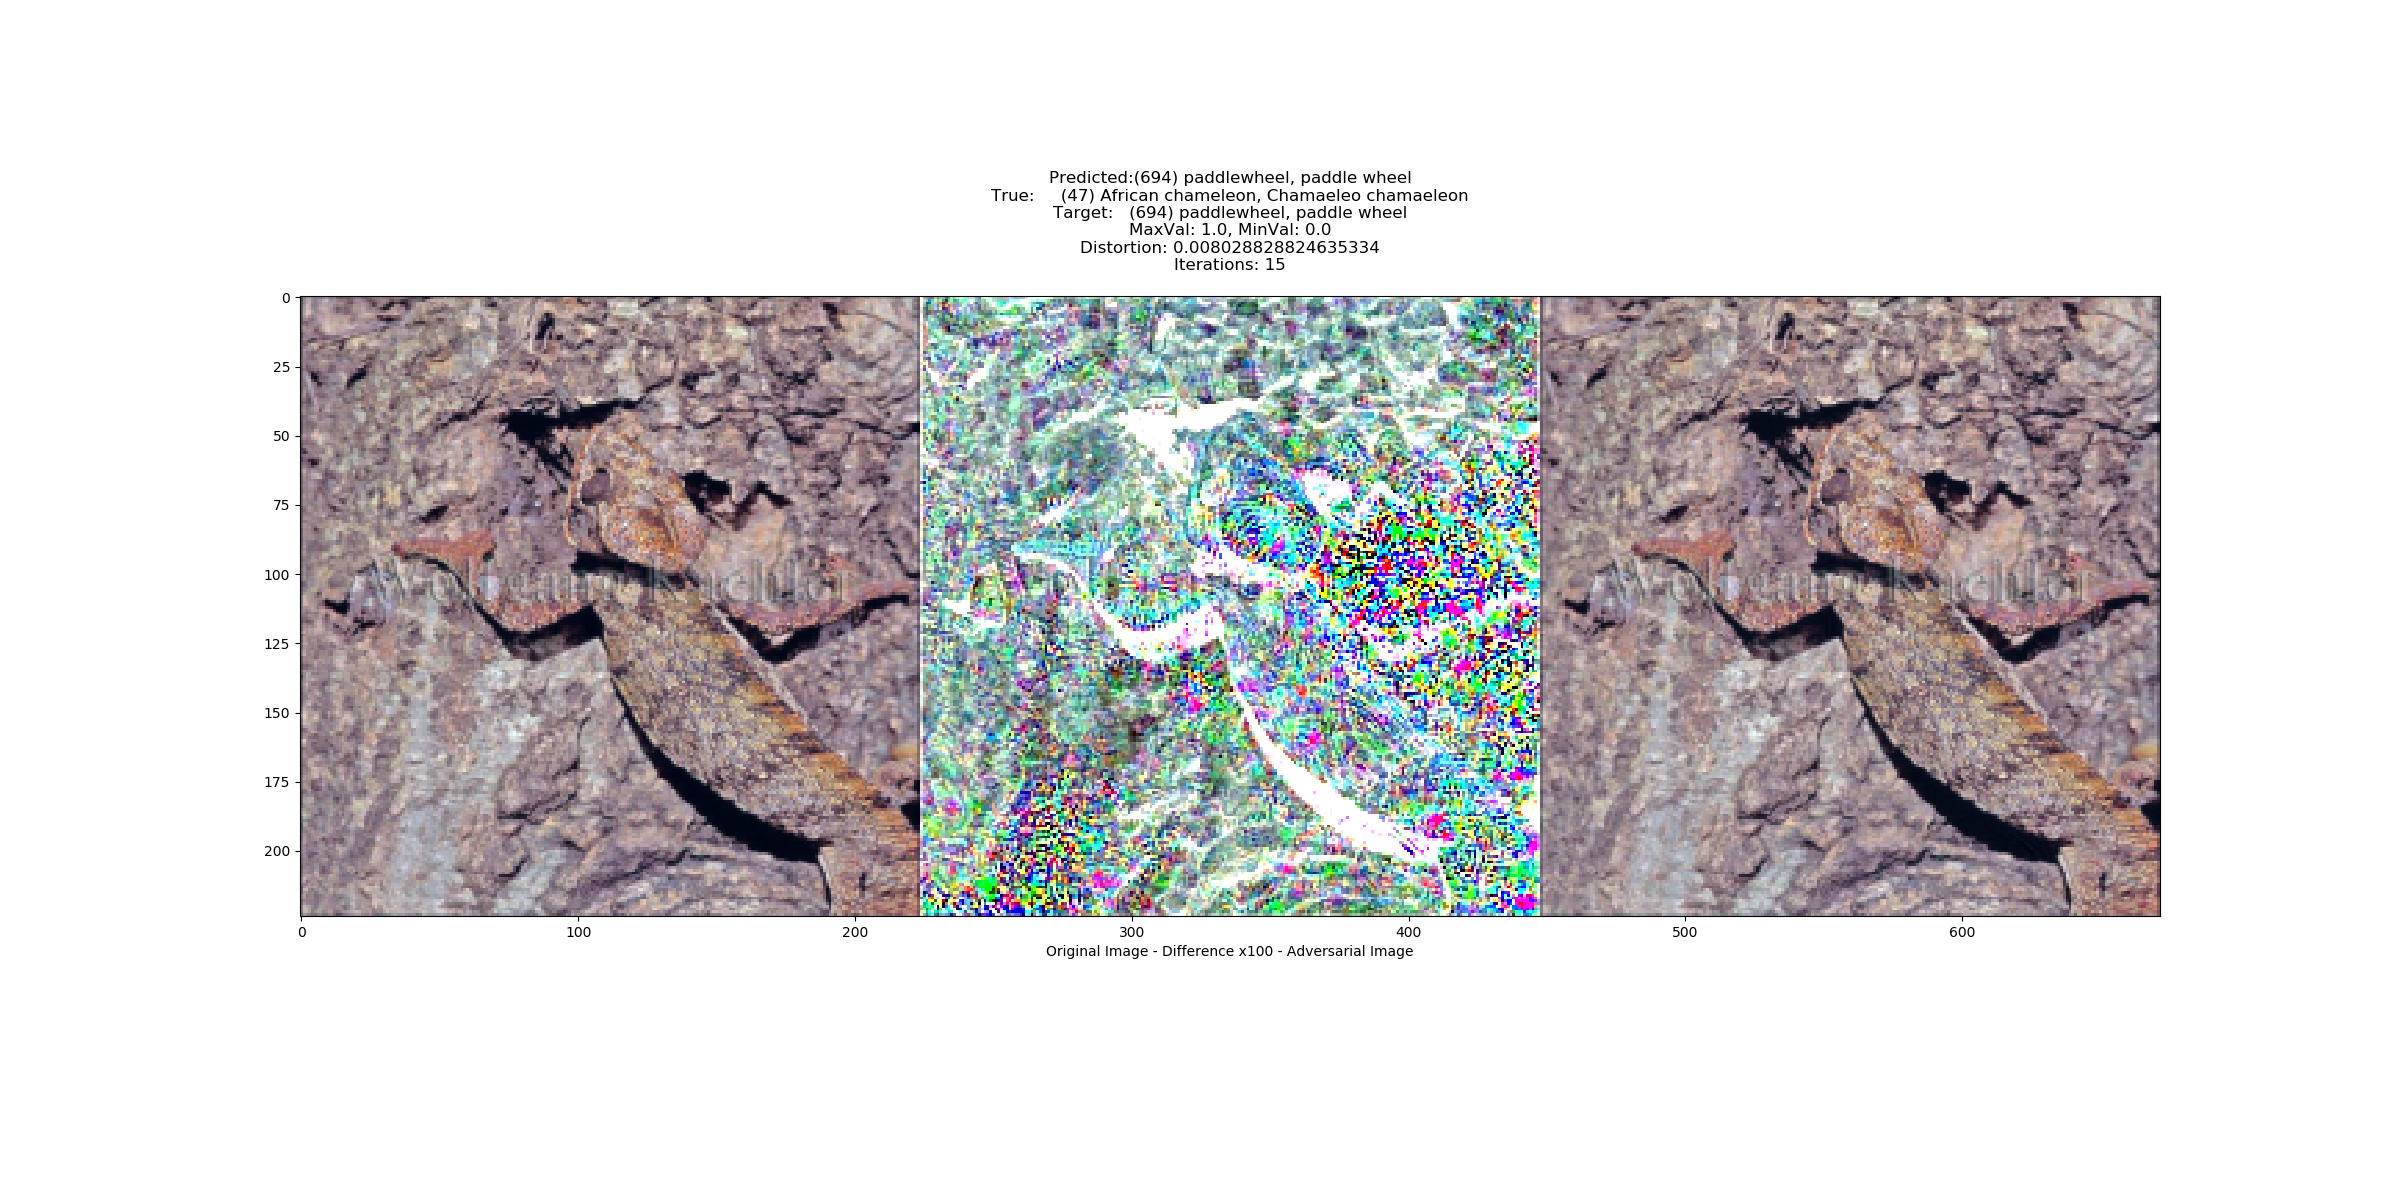
\includegraphics[trim=200 185 100 200, clip, width=8cm]{c1_figures/ILSVRC2012_val_00001375-Otensor([42])-A694-attack_summary.png}
% 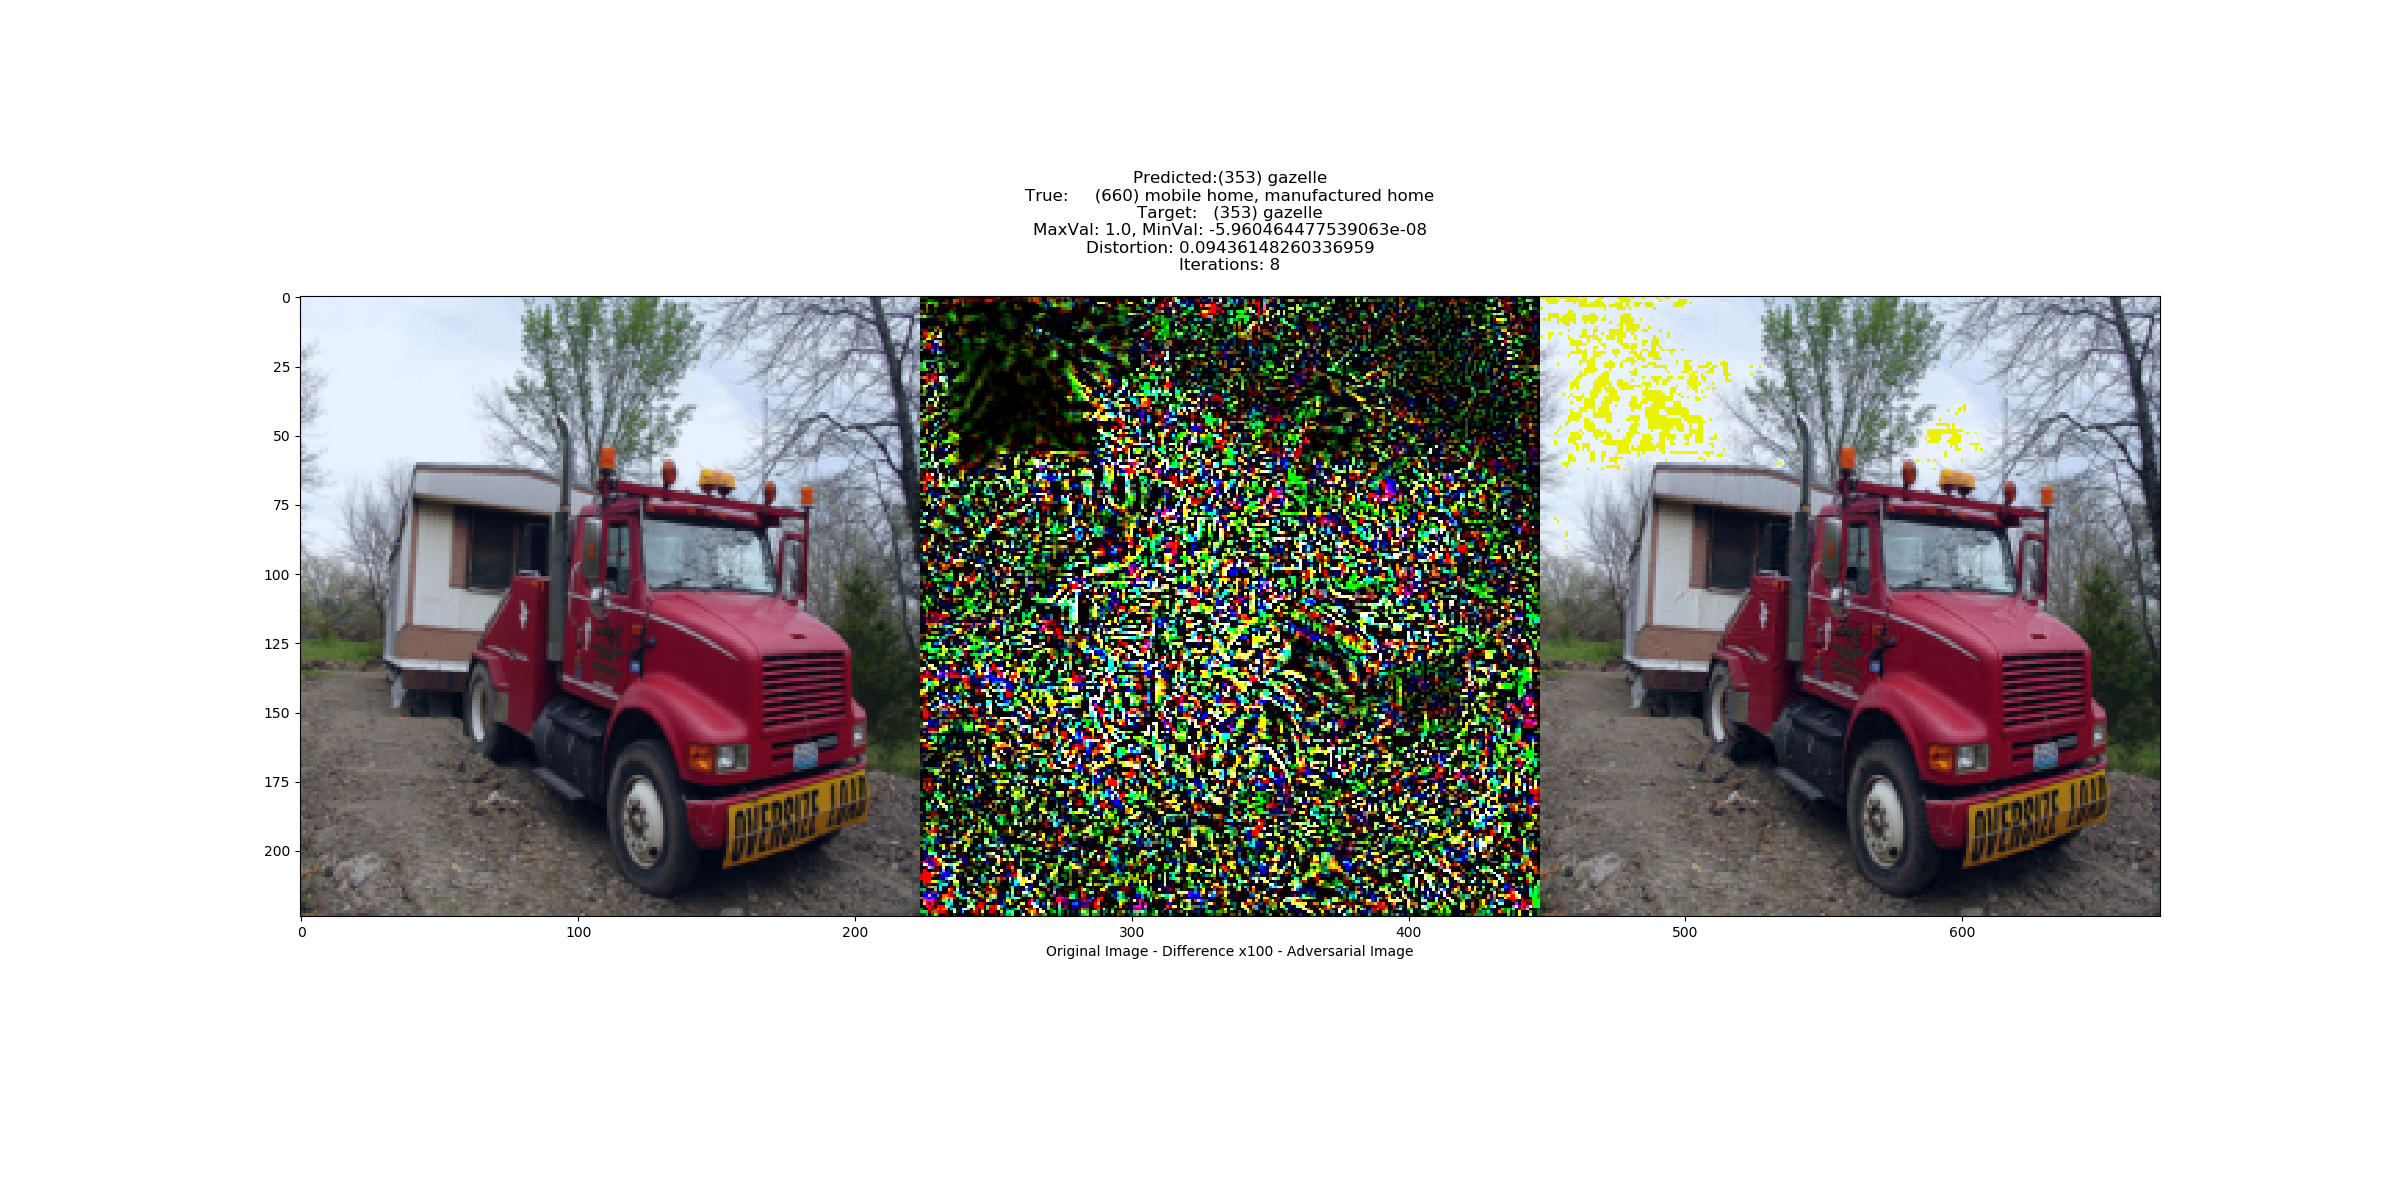
\includegraphics[width=7cm]{c1_figures/vgg16-ILSVRC2012_val_00035978-O803-A353-attack_summary.png}
% 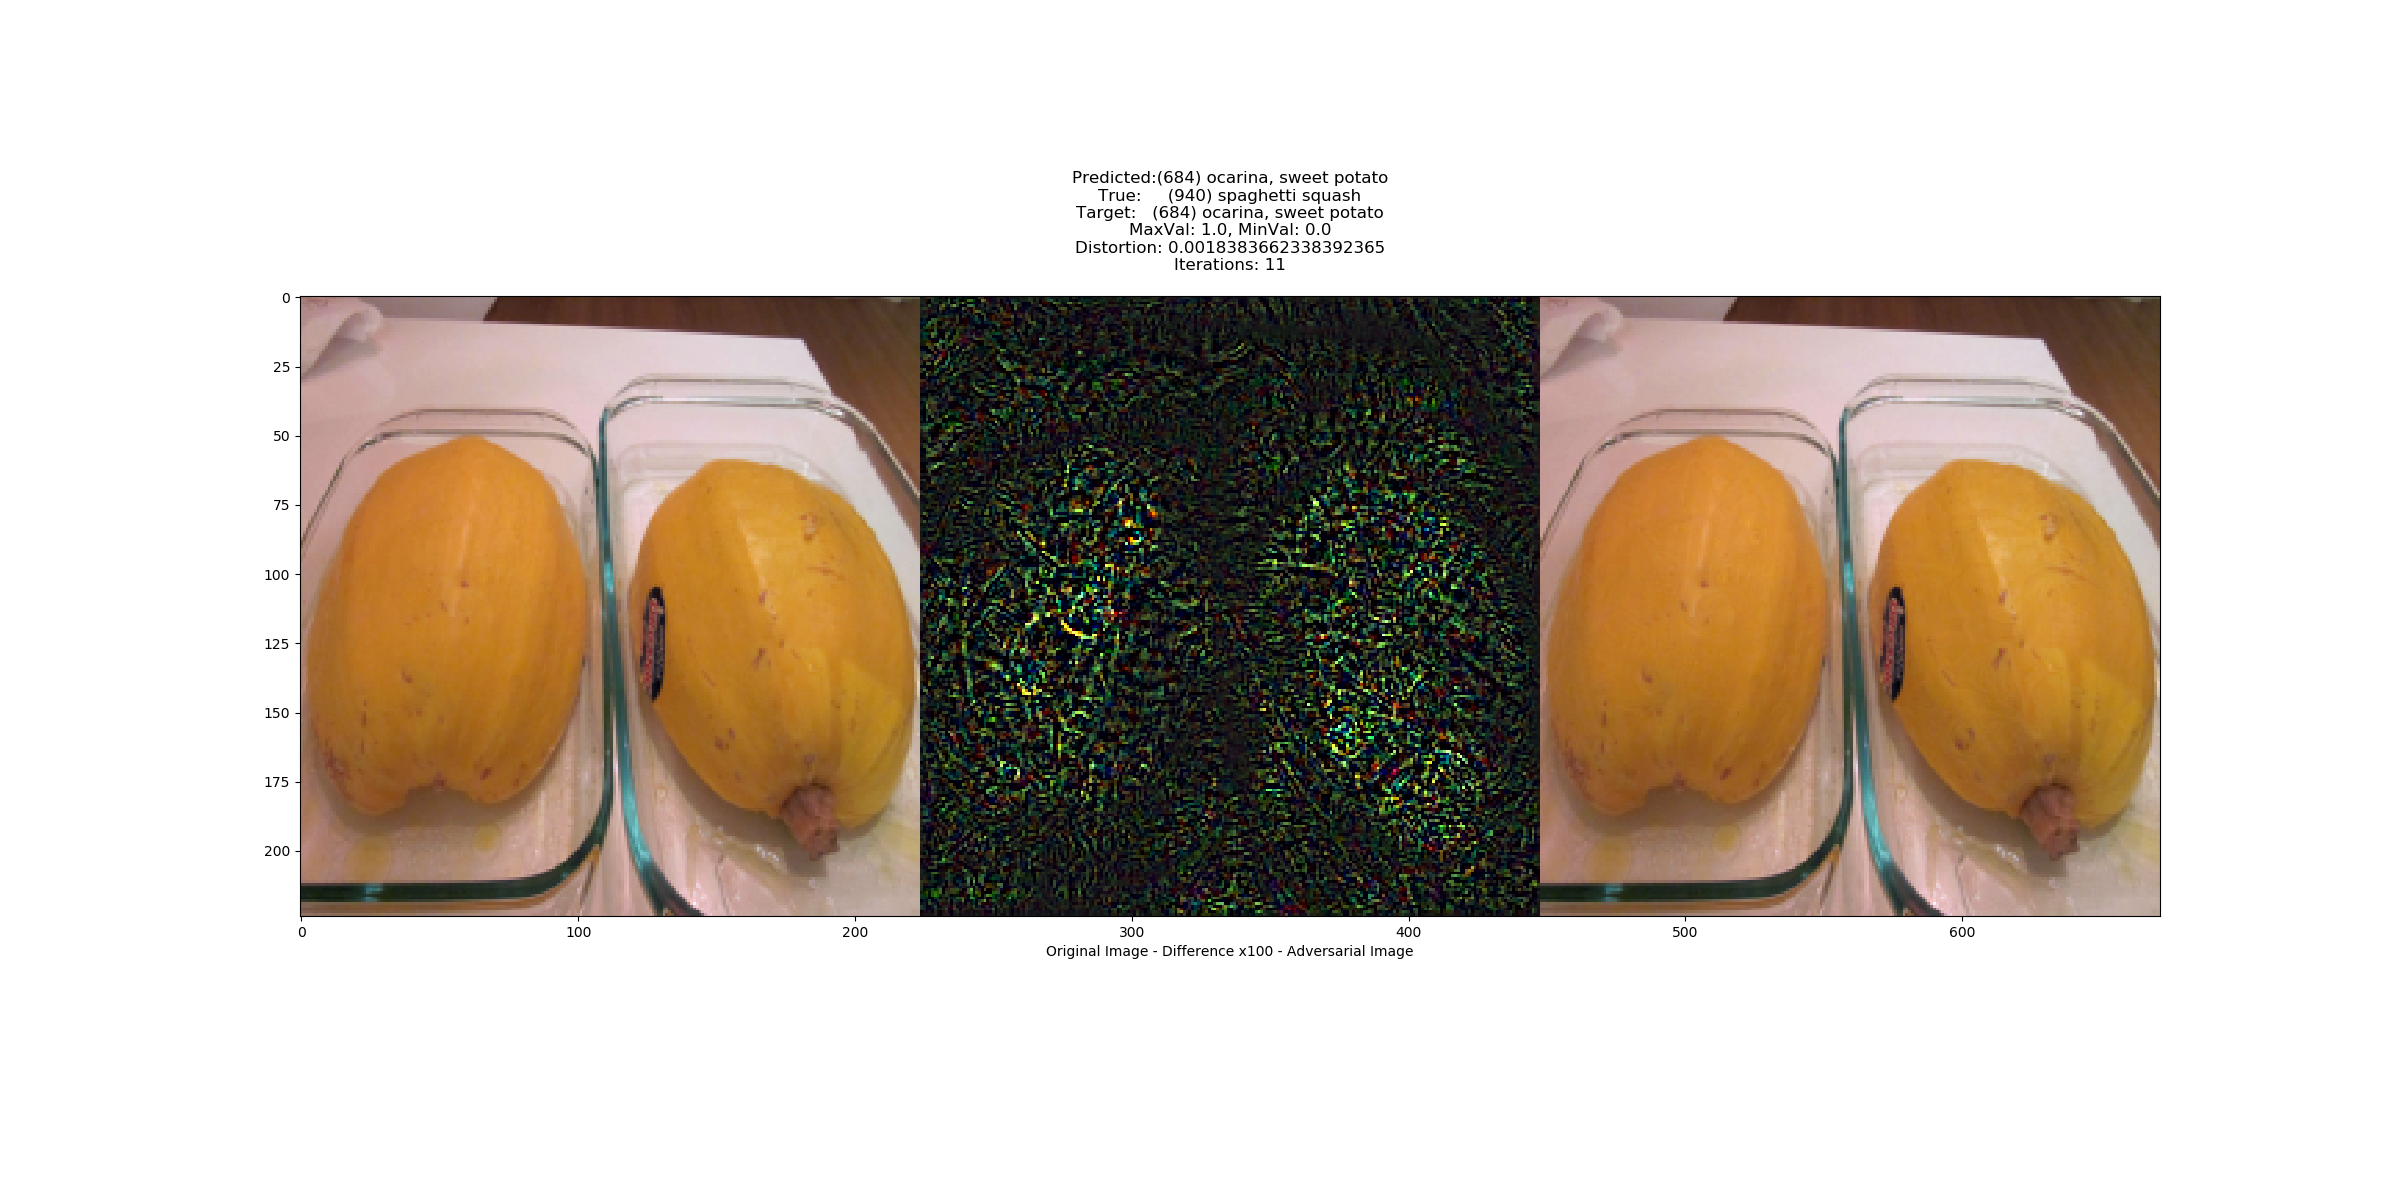
\includegraphics[width=7cm]{c1_figures/ILSVRC2012_val_00000886-Otensor([940])-A684-attack_summary.png}
\caption{Original images on the left, Perturbation (magnified by a factor of 100) by is in the middle, Adversarial Image (total of Original with Perturbation) is on the right. }
\end{figure}

%The average distortion was 0.01 distributed as seen in figure \ref{lbfgsi}. 

\begin{figure}[H]
\label{lbfgsi}
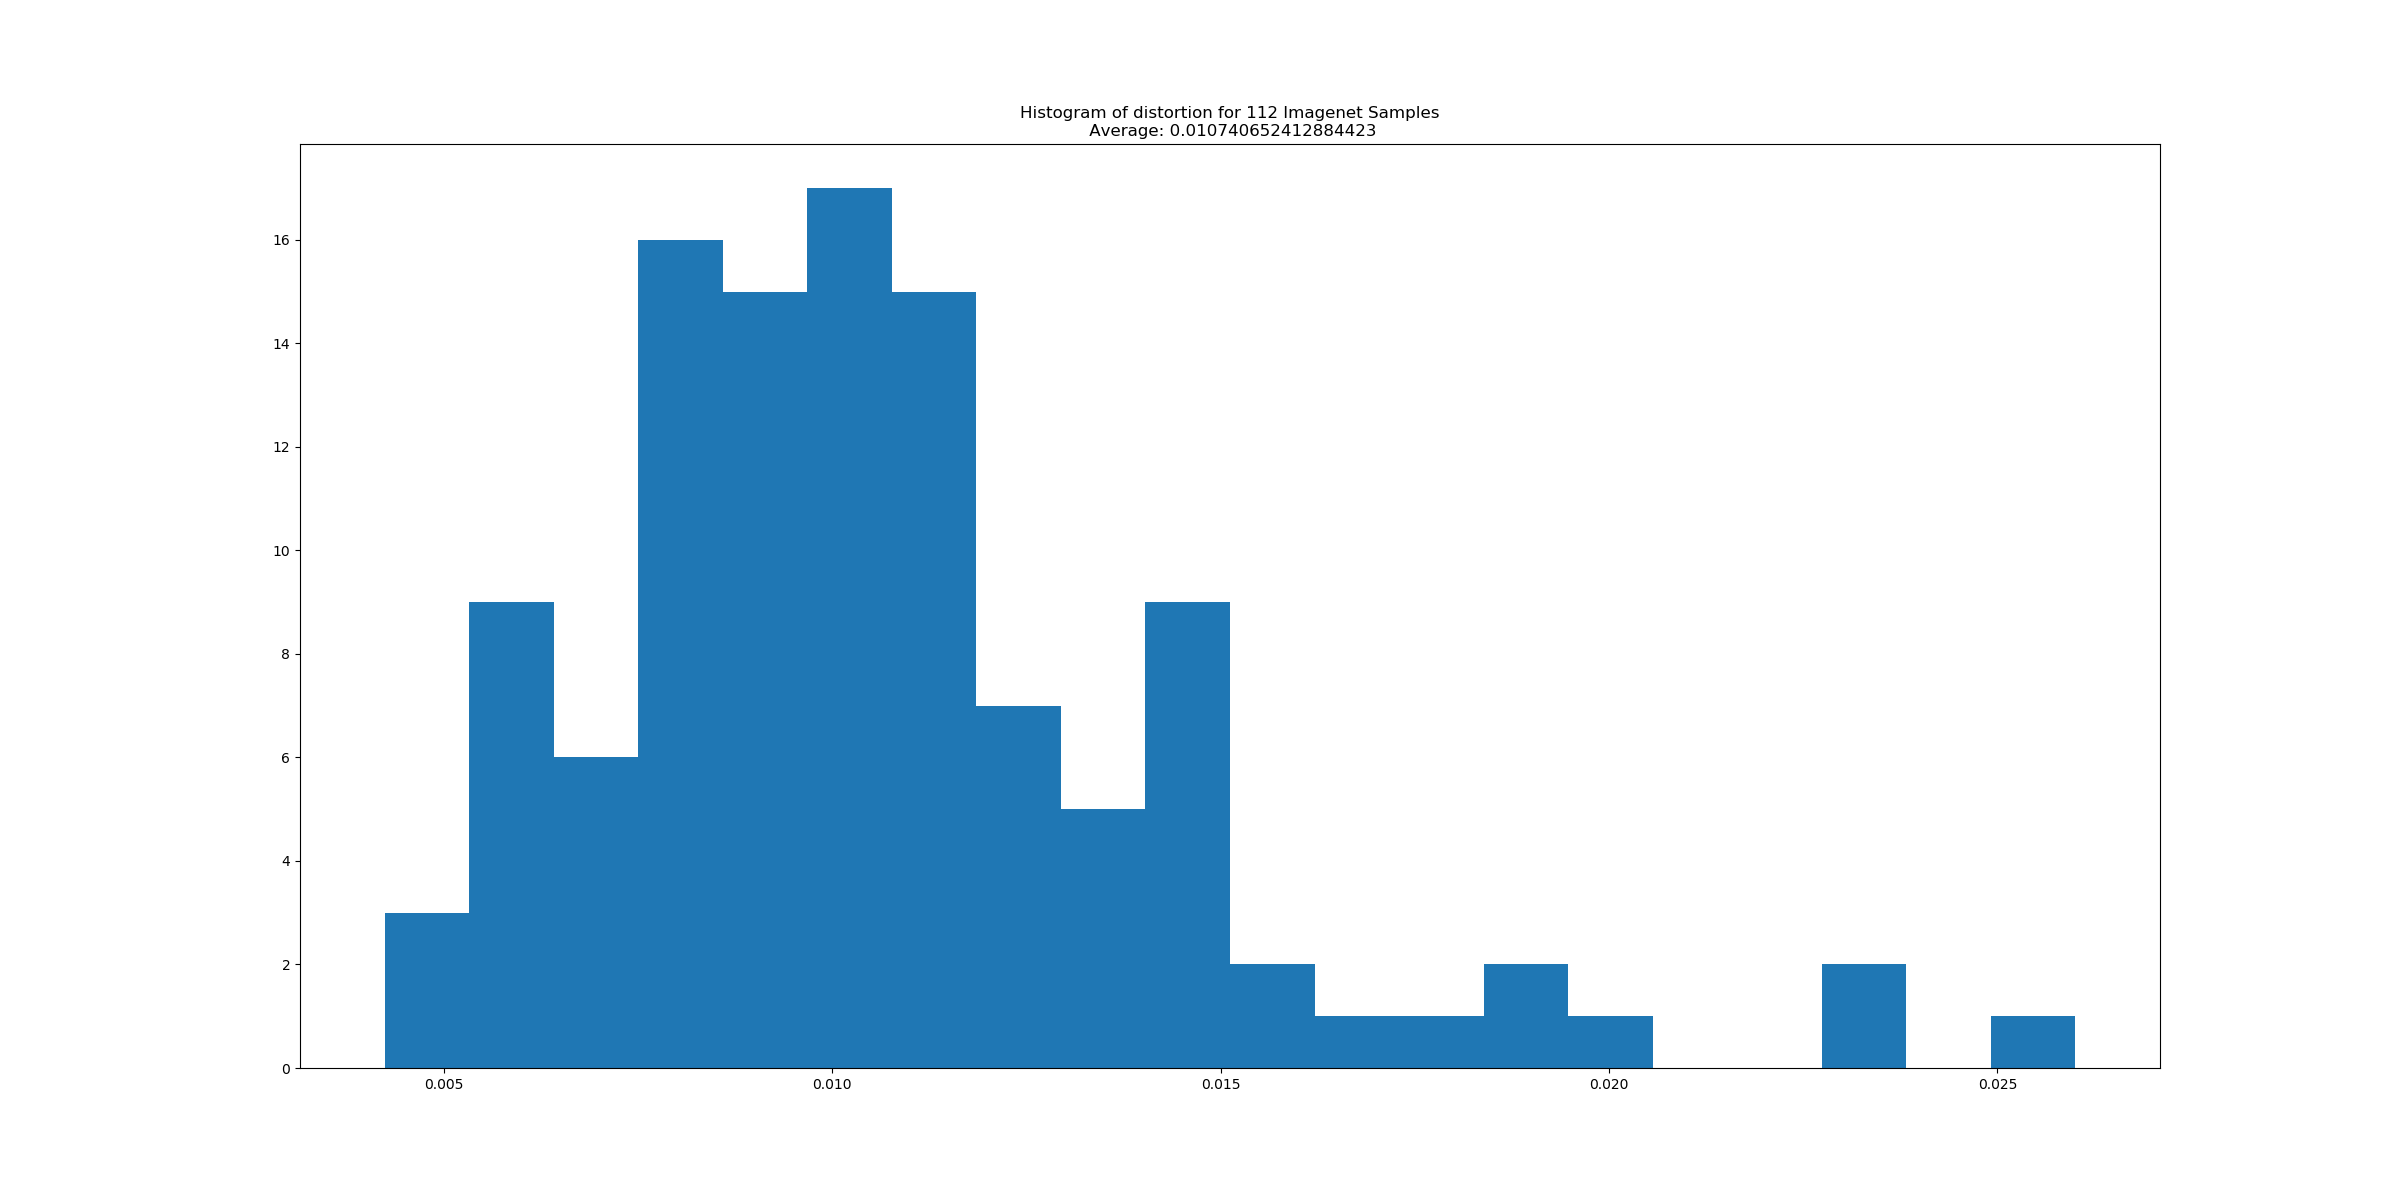
\includegraphics[trim=200 80 100 100, clip,width=14cm]{c1_figures/distortion_hist.png}
\caption{A histogram of the distortion measured for each of 112 adversarial examples generated using L-BFGS against the VGG16 network on ImageNet images with mean distortion 0.0107}
\end{figure}

\paragraph{Fast Gradient Sign Method (FGSM)} 

  We also implemented a single step attack process uses the gradient of the loss function $L$ with respect to the image to find the adversarial perturbation \cite{goodfellow_explaining_2014}. for given $\e$, the modified image $\hat x$ is computed as
\begin{equation}
\hat{x} = x + \epsilon \text{sign} (\nabla L (P_w(x),x))
\end{equation}

This method is simpler and much faster to compute than the L-BFGS technique described above, but produces adversarial examples less reliably and with generally larger distortion. Performance was similar but inferior to the Iterative Gradient Sign Method summarized below.  
%\[\hat x = x + \e \sign(\Delta \ell(F(x'_m),x'_m))\]

\paragraph{Iterative Gradient Sign Method (IGSM)}
\label{igsm-s}
In \cite{kurakin_adversarial_2016}
  an iterative application of FGSM was proposed. After each
  iteration, the image is clipped to a $\e L_\infty$ neighborhood of the original. Let $x'_0 = x$, then after $m$ iterations, the adversarial image obtained is:
\begin{equation}
x_{m+1}' = \text{Clip}_{x,\epsilon} \Bigl\{x_m' + \alpha \times \text{sign}(\nabla \ell (F(x'_m),x'_m))  \Bigr\} 
\label{igsm}
\end{equation}
This method is faster than L-BFGS and more reliable than FGSM but still produces examples with greater distortion than L-BFGS. 
%  \[x'_{m + 1} = \text{Clip}_{x,\e} \{ x'_m + \alpha \times
%  \sign(\Delta \ell(F(x'_m),x'_m))\] 
\begin{figure}[H]
  \centering
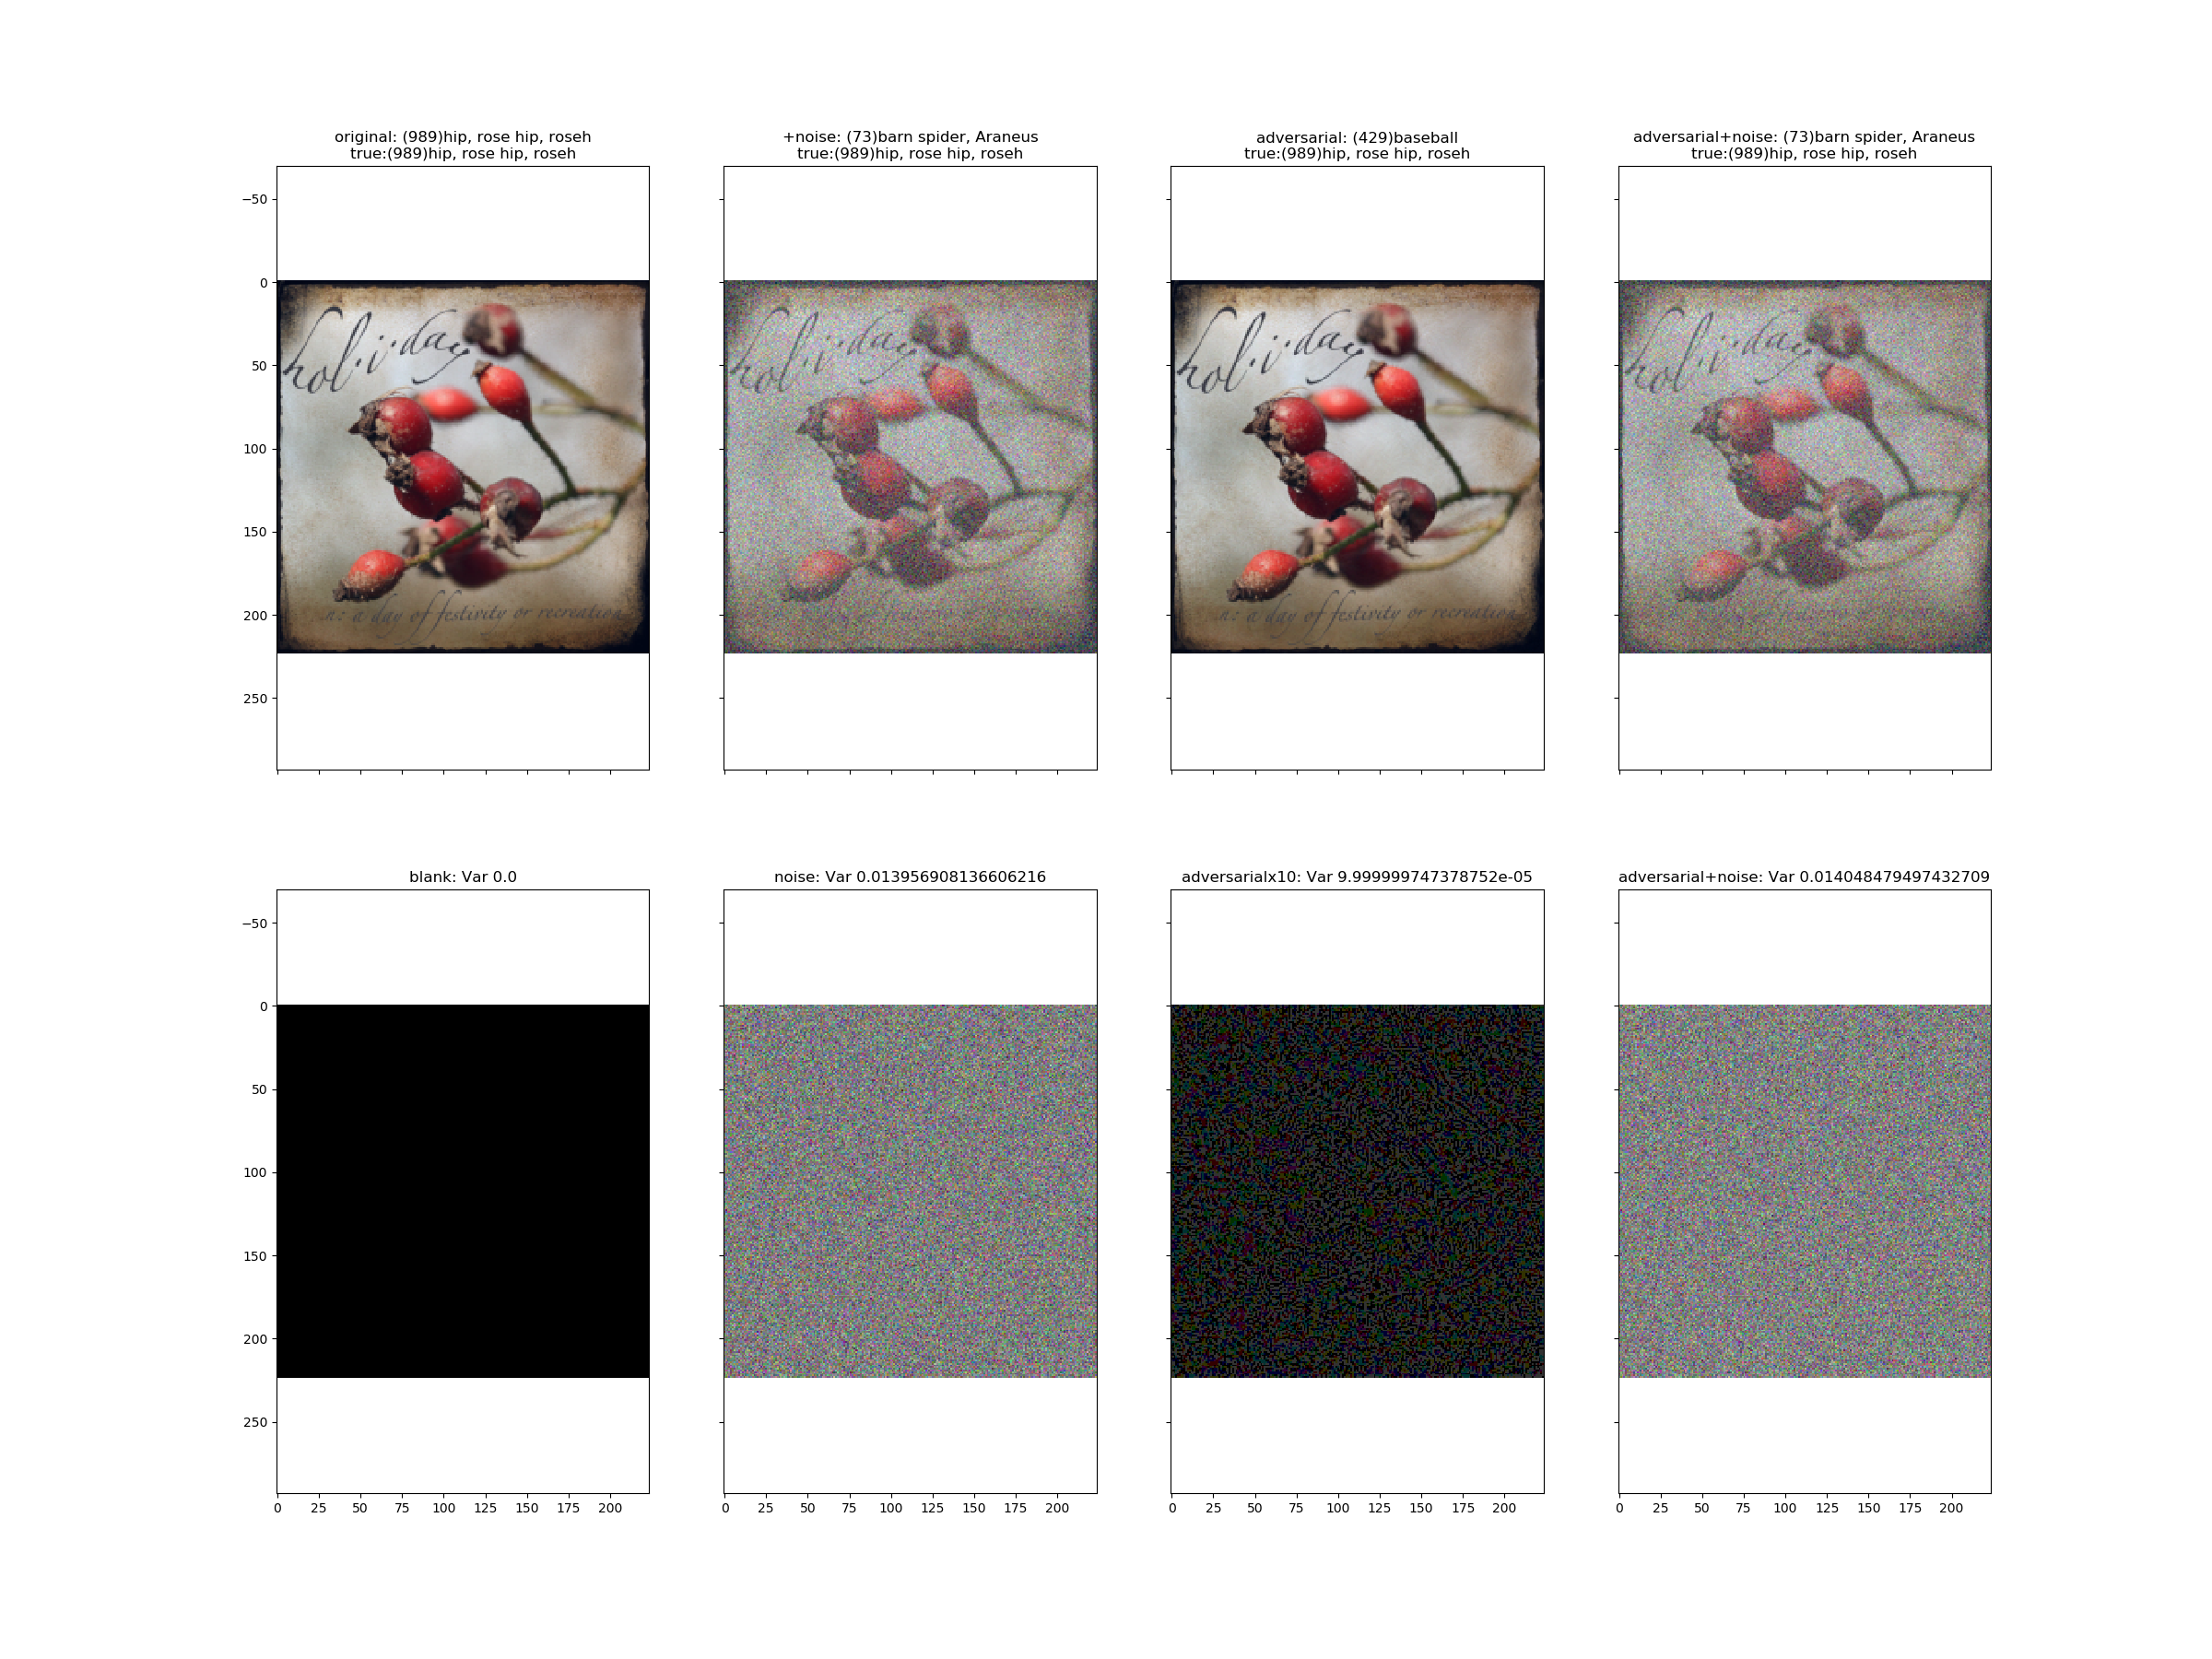
\includegraphics[trim=200 110 1200 102, clip,width=4cm]{c1_figures/ILSVRC2012_val_00002900summary_plot.png}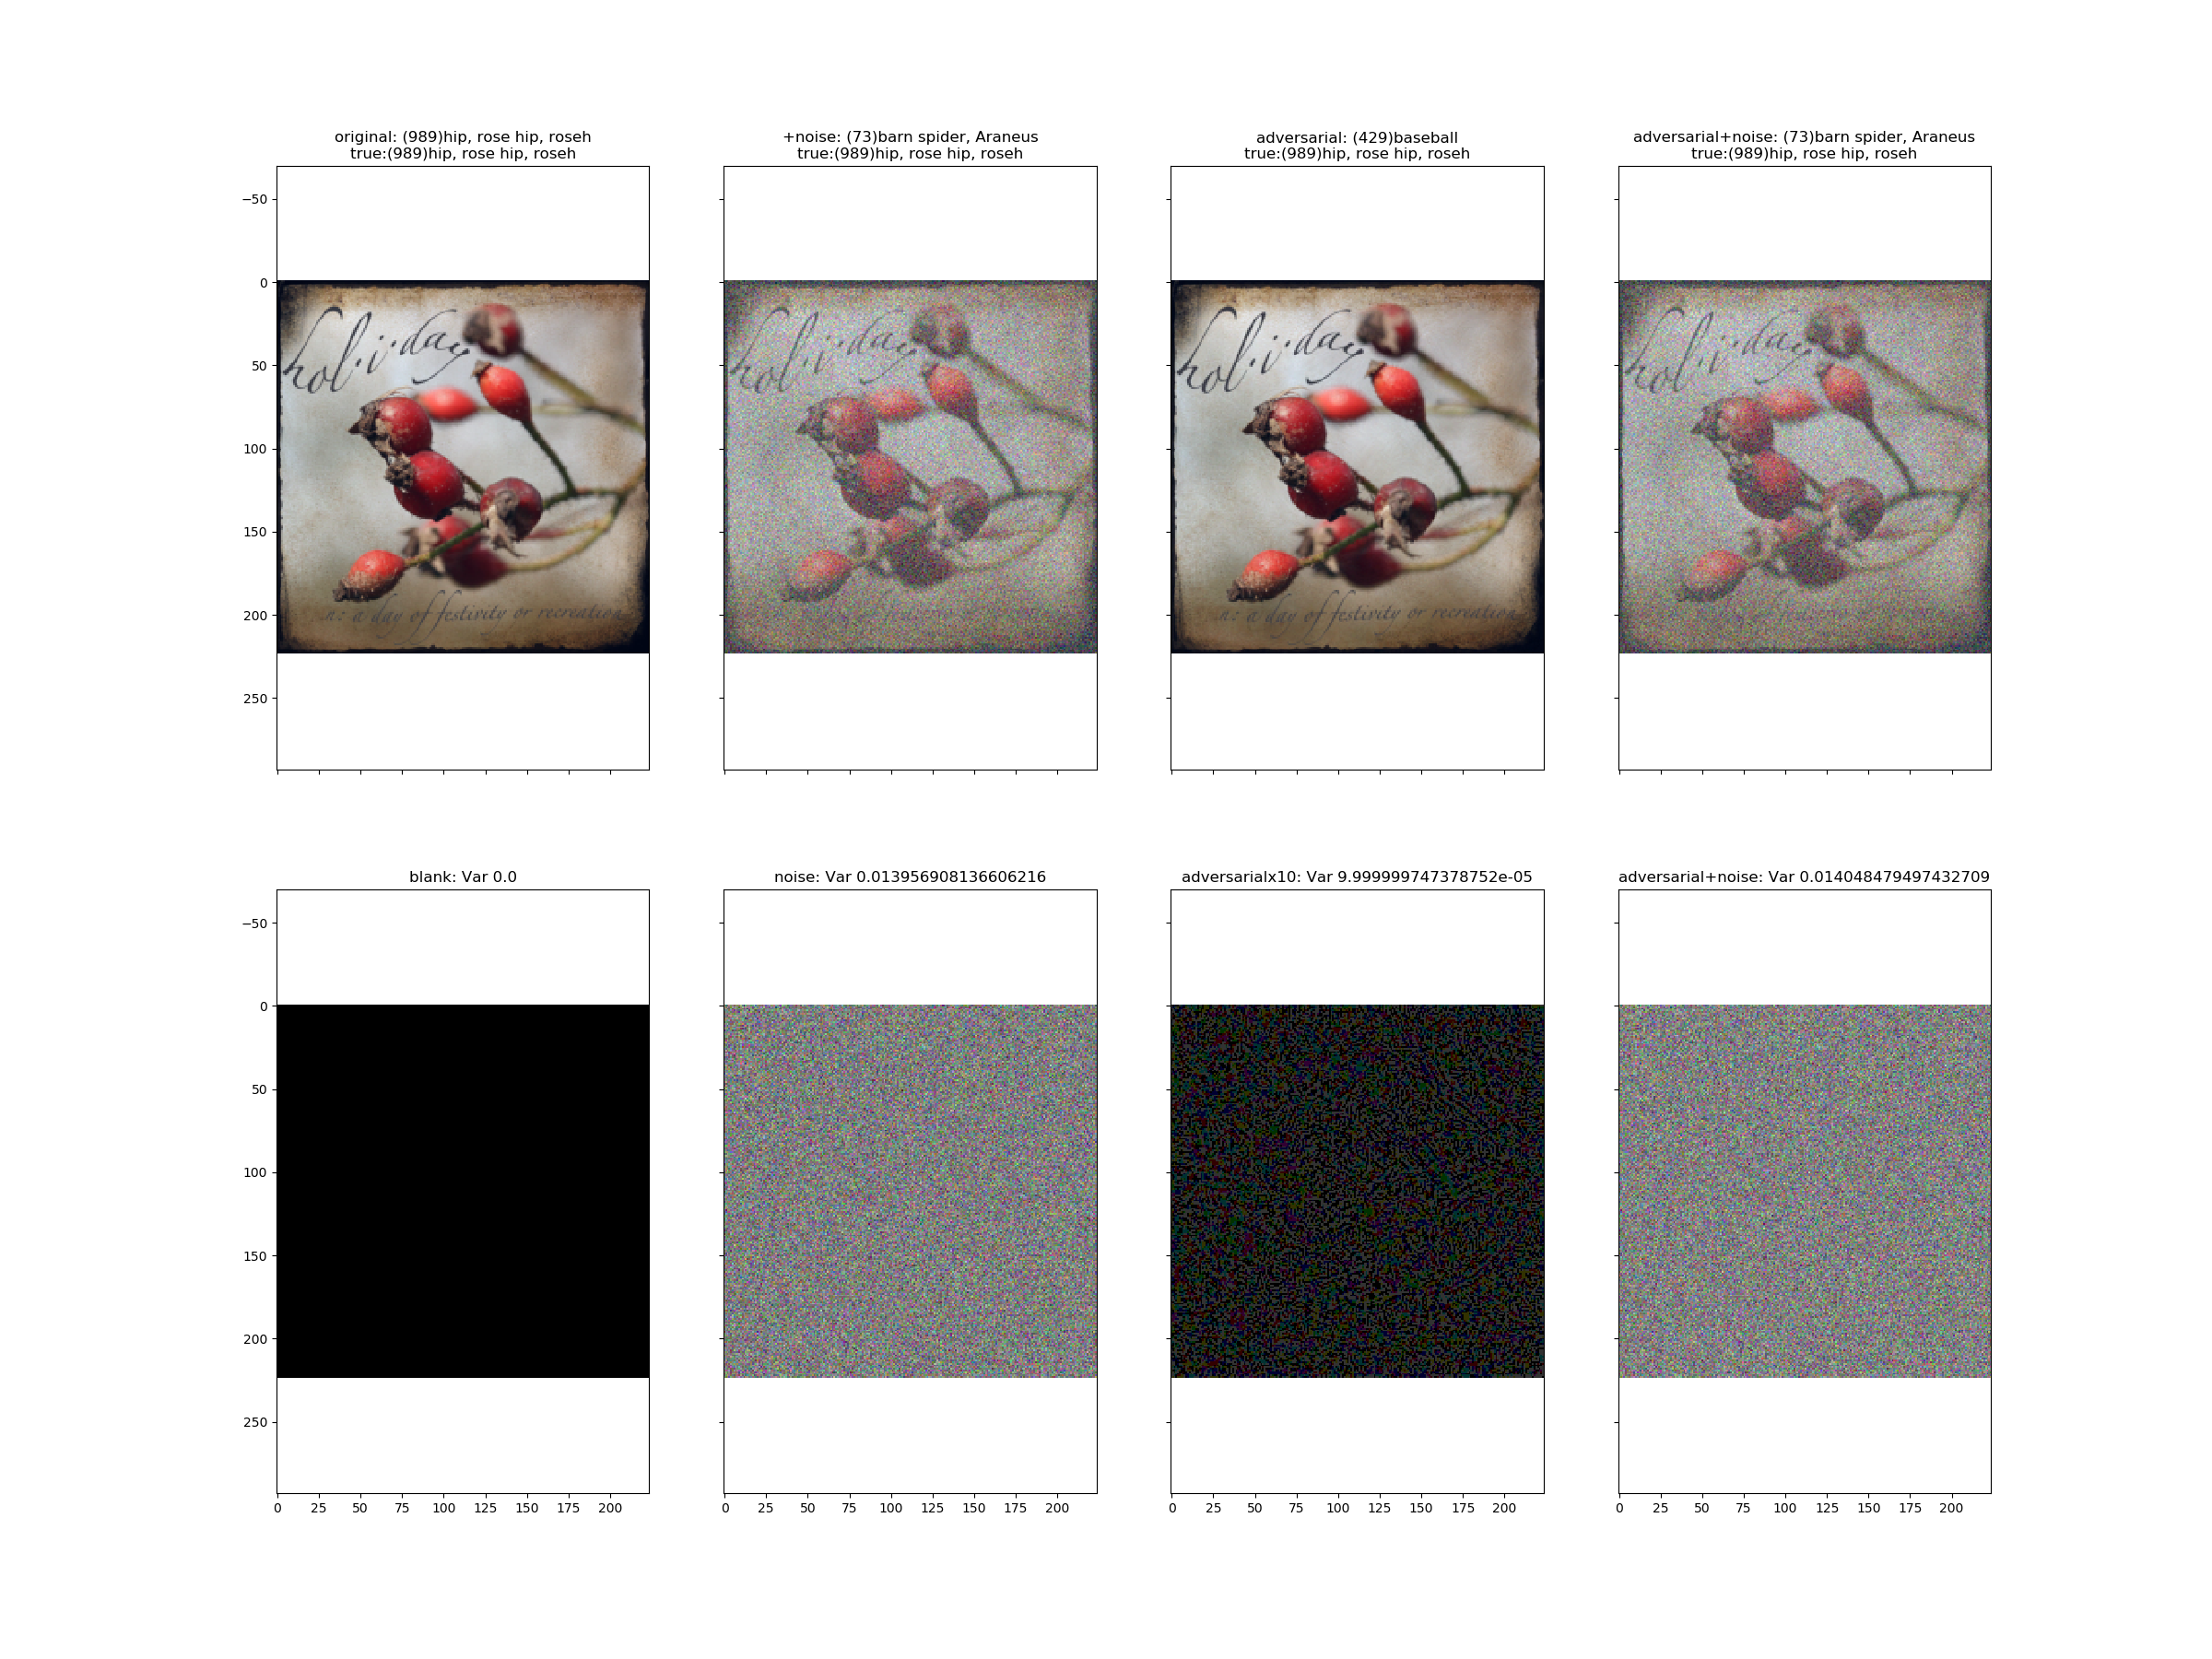
\includegraphics[trim=900 110 500 102, clip,width=4cm]{c1_figures/ILSVRC2012_val_00002900summary_plot.png}
%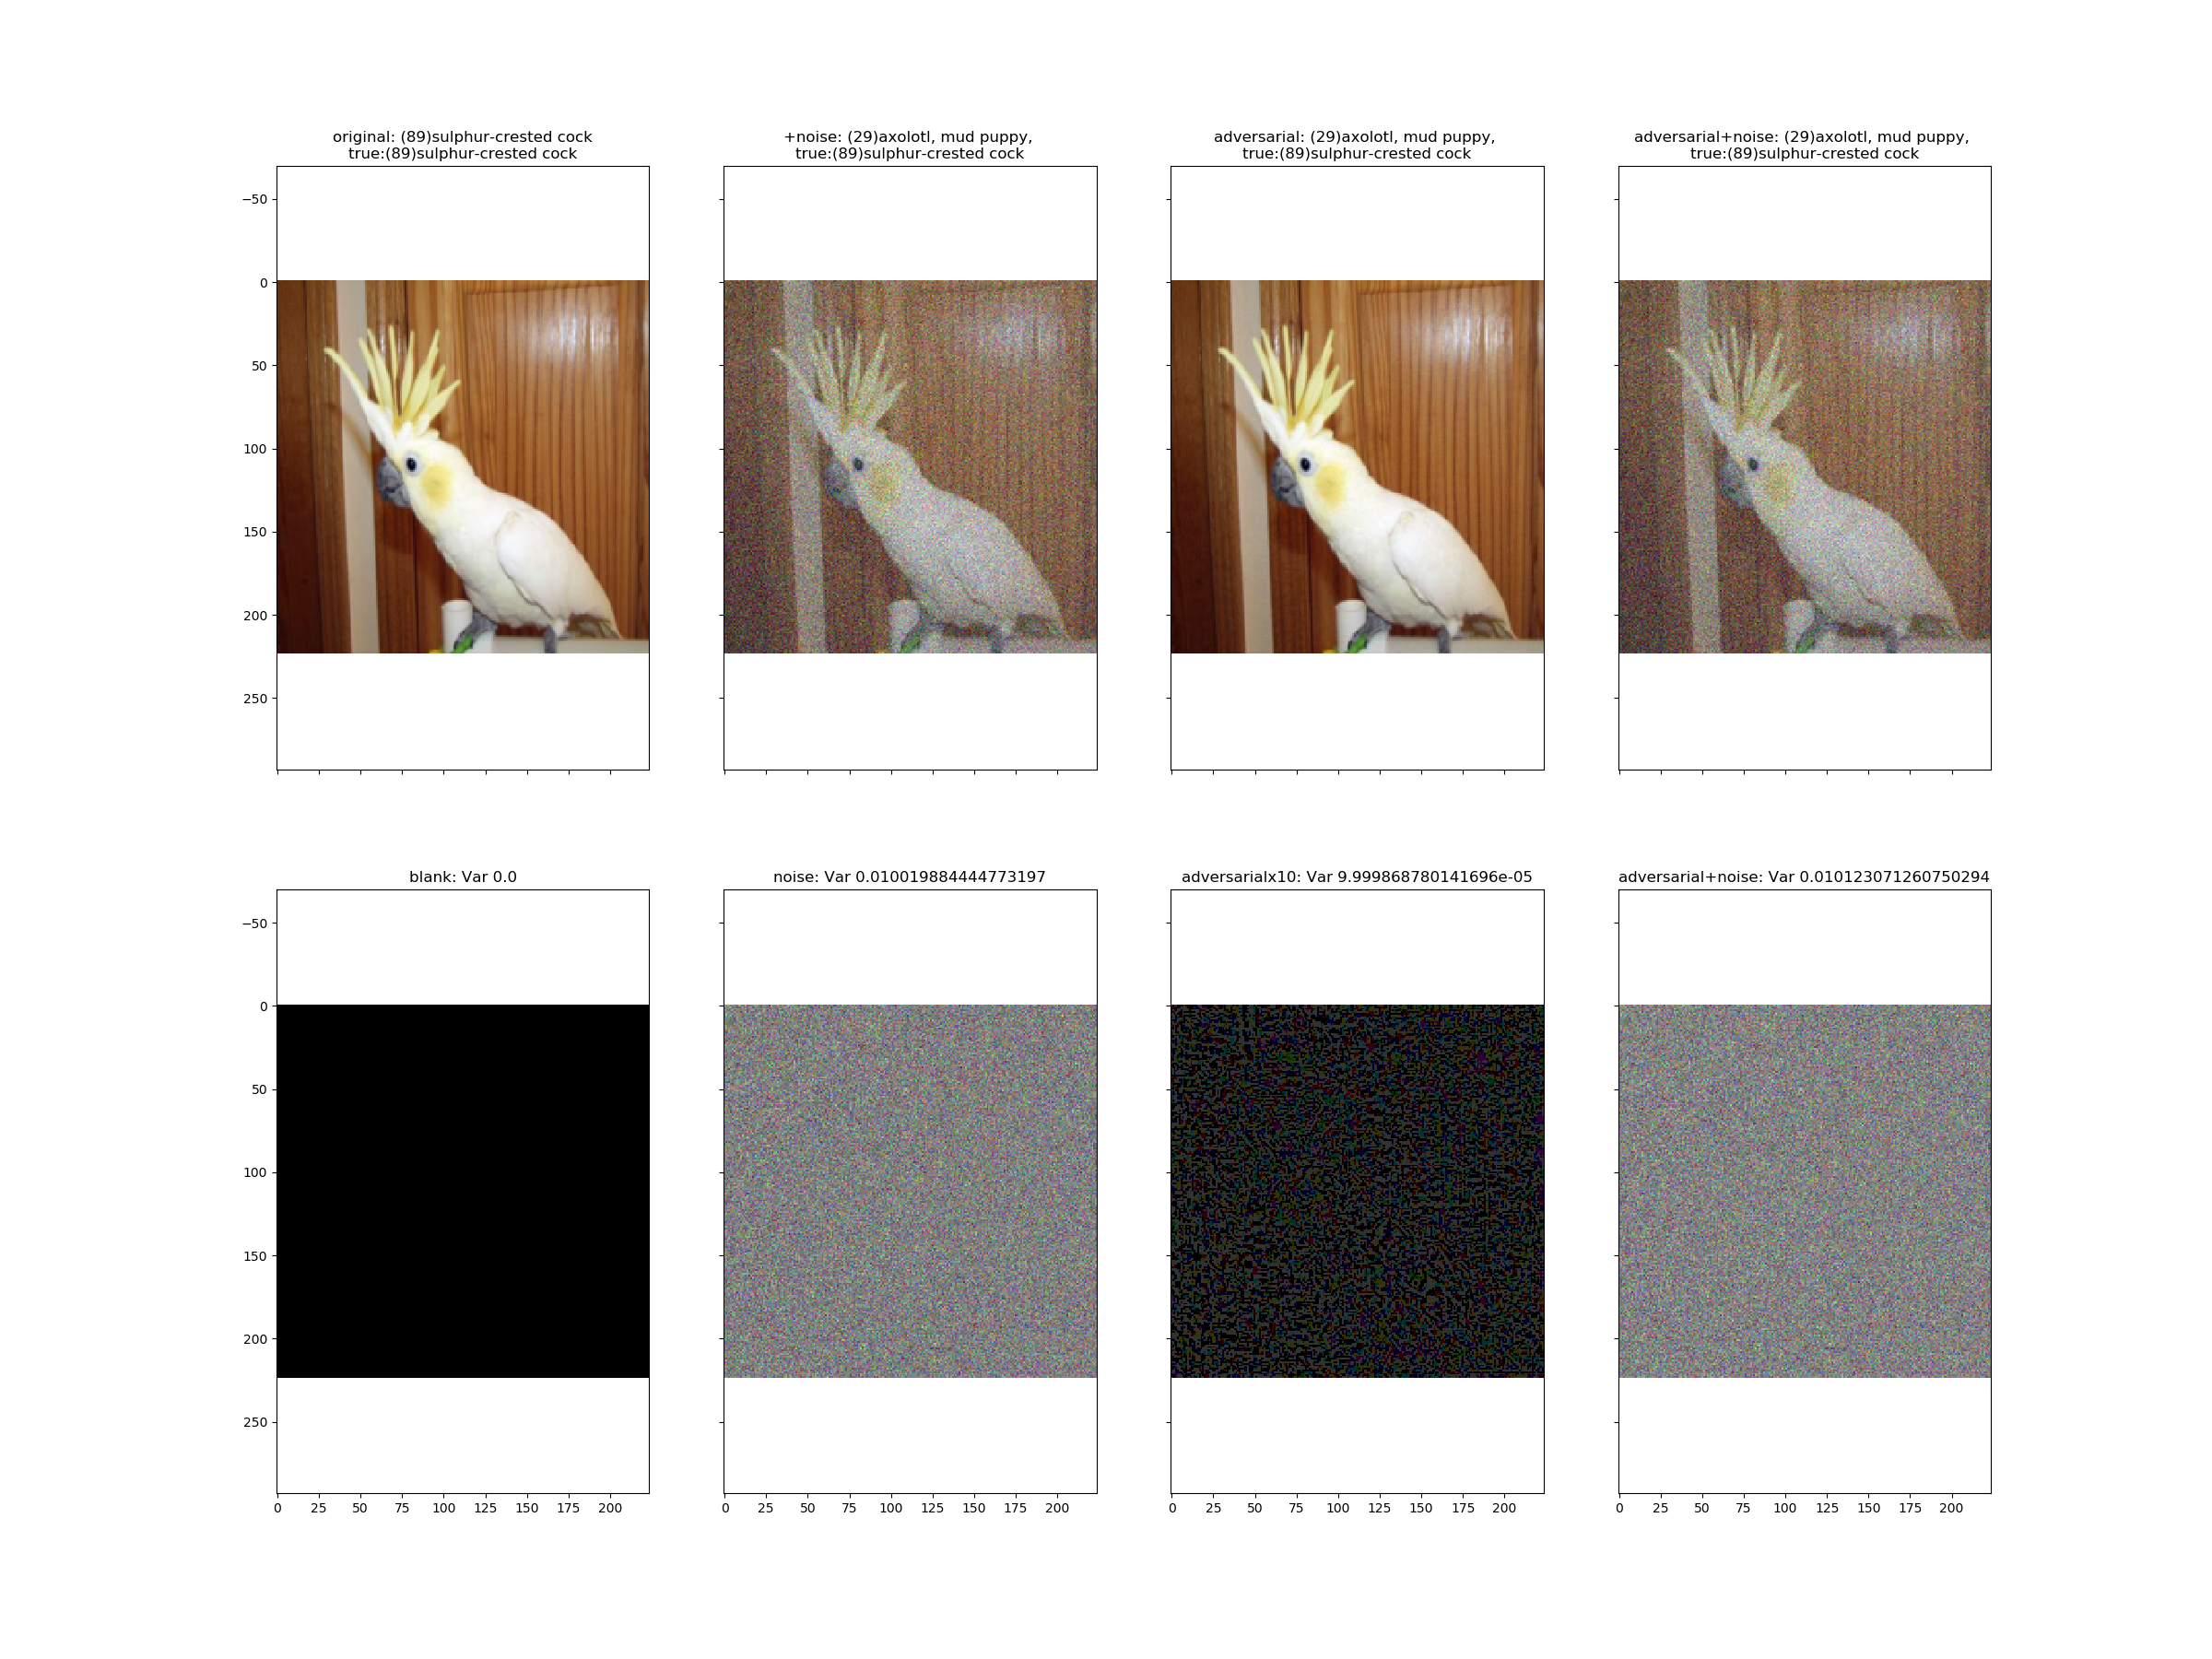
\includegraphics[width=12cm]{c1_figures/ILSVRC2012_val_00048234summary_plot.png}
\label{fgsmhip}
\caption{adversarial example generated against VGG16 (ImageNet) with IGSM. Original Image on the left, adversarial image and added noise (ratio of variance adversarial noise/original image: 0.0000999) on the right. }
\end{figure}

%The attacks contained in figure ~\ref{fgsmhip} were generated with IGSM against VGG16


\subsubsection{Other Attacks}
The following attack techniques are also prevalent in the literature but have not been replicated in these experiments. 

\paragraph{Jacobian-based Saliency Map Attack (JSMA)} Another attack noted by  \cite{papernot_limitations_2015}
  estimates the \emph{saliency map}, a rating for each of the input features (e.g. each pixel) on how influential it is for causing the model to predict a particular class with respect to the model output \cite{wiyatno2018saliency}. This attack modifies the pixels that are most salient. This is a targeted attack, and saliency is designed to find the pixel which increases the classifier's output for the target class while tending to decrease the output for other classes.

\paragraph{Deep Fool (DFool)} A technique proposed by \cite{moosavi-dezfooli_deepfool:_2015}
  to generate an un-targeted iterative attack. 
This method approximates the classifier as a linear decision boundary and then finds the smallest perturbation needed to cross that boundary.
This attack minimizes $L_2$ norm with respect to  to the original image.

\paragraph{Carlini \& Wagner (C\&W)} In \cite{carlini_towards_2016}
  an adversarial attack is proposed which updates the loss function such that it jointly minimizes $L_p$ and a custom differentiable loss function based on un-normalized outputs of the classifier (\textit{logits}). 
Let $Z_k$ denote the logits of a model for a given class $k$, and $\kappa$ a margin parameter. Then C\&W tries to minimize:
\begin{equation}
|| x - \hat{x} ||_p + c* max\left(Z_k(\hat{x}_y) - max\{Z_k(\hat{x}) : k \neq y\},-\kappa\right)
\end{equation}

